\documentclass[acmlarge,review,anonymous]{acmart}

\settopmatter{printfolios=true}

\bibliographystyle{ACM-Reference-Format}
\citestyle{acmauthoryear}

\usepackage[english]{babel}
\usepackage{setspace}

\usepackage{paralist}
\usepackage{tikz}
\usetikzlibrary{arrows}

\usepackage{isabelle,isabellesym}
\isabellestyle{it}

\hyphenation{App-Jet}

%% PACMPL journal information will be supplied by publisher for camera-ready submission
\acmJournal{PACMPL}
\acmVolume{--}
\acmNumber{--}
\acmArticle{0}
\acmYear{2017}
\acmMonth{4}
\acmDOI{10.1145/nnnnnnn.nnnnnnn}
\startPage{1}
\setcopyright{none}

\widowpenalty=2000
\clubpenalty=2000

\begin{document}
\title{Verifying Strong Eventual Consistency in Distributed Systems}

%% Each author should be introduced by \author, followed by \authornote (optional),
%% \orcid (optional), \affiliation, and \email.
%% An author may have multiple affiliations and/or emails; repeat the appropriate command.
%% Many elements are not rendered, but should be provided for metadata extraction tools.
\author{Victor B.\ F.\ Gomes}
\orcid{0000-0002-2954-4648}
\affiliation{
  \position{Research Associate}
  \department{Computer Laboratory}
  \institution{University of Cambridge}
  \streetaddress{15 JJ Thomson Avenue}
  \city{Cambridge}
  \postcode{CB3 0FD}
  \country{UK}
}
\email{vb358@cam.ac.uk}

\author{Martin Kleppmann}
\orcid{0000-0001-7252-6958}
\affiliation{
  \position{Research Associate}
  \department{Computer Laboratory}
  \institution{University of Cambridge}
  \streetaddress{15 JJ Thomson Avenue}
  \city{Cambridge}
  \postcode{CB3 0FD}
  \country{UK}
}
\email{mk428@cam.ac.uk}

\author{Dominic P.\ Mulligan}
\orcid{0000-0003-4643-3541}
\affiliation{
  \position{Research Associate}
  \department{Computer Laboratory}
  \institution{University of Cambridge}
  \streetaddress{15 JJ Thomson Avenue}
  \city{Cambridge}
  \postcode{CB3 0FD}
  \country{UK}
}
\email{dpm36@cam.ac.uk}

\author{Alastair R.\ Beresford}
\orcid{0000-0003-0818-6535}
\affiliation{
  \position{Senior Lecturer}
  \department{Computer Laboratory}
  \institution{University of Cambridge}
  \streetaddress{15 JJ Thomson Avenue}
  \city{Cambridge}
  \postcode{CB3 0FD}
  \country{UK}
}
\email{arb33@cam.ac.uk}

\begin{abstract}
Data replication is used in distributed systems to maintain up-to-date copies of shared data across multiple computers in a network.
However, despite decades of research, algorithms for achieving consistency in replicated systems are still poorly understood.
Indeed, many published algorithms have later been shown to be incorrect, even some that were accompanied by supposed mechanised proofs of correctness.
In this work, we focus on the correctness of Conflict-free Replicated Data Types (CRDTs), a class of algorithm that provides strong eventual consistency guarantees for replicated data.
We develop a modular and reusable framework in the Isabelle/HOL interactive proof assistant for verifying the correctness of CRDT algorithms.
We avoid correctness issues that have dogged previous mechanised proofs in this area by including a network model in our formalisation, and proving that our theorems hold in all possible network behaviours.
Our axiomatic network model is a standard abstraction that accurately reflects the behaviour of real-world computer networks.
Moreover, we identify an abstract convergence theorem, a property of order relations, which provides a formal definition of strong eventual consistency.
We then obtain the first machine-checked correctness theorems for three concrete CRDTs: the Replicated Growable Array, the Observed-Remove Set, and an Increment-Decrement Counter.
We find that our framework is highly reusable, developing proofs of correctness for the latter two CRDTs in a few hours and with relatively little CRDT-specific code.
\end{abstract}

\begin{CCSXML}
<ccs2012>
<concept>
<concept_id>10003033.10003039.10003041.10003042</concept_id>
<concept_desc>Networks~Protocol testing and verification</concept_desc>
<concept_significance>500</concept_significance>
</concept>
<concept>
<concept_id>10010520.10010521.10010537.10010540</concept_id>
<concept_desc>Computer systems organization~Peer-to-peer architectures</concept_desc>
<concept_significance>500</concept_significance>
</concept>
<concept>
<concept_id>10003033.10003039.10003041.10003043</concept_id>
<concept_desc>Networks~Formal specifications</concept_desc>
<concept_significance>300</concept_significance>
</concept>
<concept>
<concept_id>10003752.10003809.10010172</concept_id>
<concept_desc>Theory of computation~Distributed algorithms</concept_desc>
<concept_significance>300</concept_significance>
</concept>
<concept>
<concept_id>10003752.10010124.10010138.10010142</concept_id>
<concept_desc>Theory of computation~Program verification</concept_desc>
<concept_significance>300</concept_significance>
</concept>
<concept>
<concept_id>10011007.10011074.10011099.10011692</concept_id>
<concept_desc>Software and its engineering~Formal software verification</concept_desc>
<concept_significance>300</concept_significance>
</concept>
</ccs2012>
\end{CCSXML}

\ccsdesc[500]{Networks~Protocol testing and verification}
\ccsdesc[500]{Computer systems organization~Peer-to-peer architectures}
\ccsdesc[300]{Networks~Formal specifications}
\ccsdesc[300]{Theory of computation~Distributed algorithms}
\ccsdesc[300]{Theory of computation~Program verification}
\ccsdesc[300]{Software and its engineering~Formal software verification}

\keywords{strong eventual consistency, verification, distributed systems, replication, convergence, CRDTs, automated theorem proving}

\maketitle


%%%%%%%%%%%%%%%%%%%%%%%%%%%%%%%%%%%%%%%%%%%%%%%%%%%%%%%%%%%%%%%%%%%%%%%%%%%%%%%%
% Introduction
%%%%%%%%%%%%%%%%%%%%%%%%%%%%%%%%%%%%%%%%%%%%%%%%%%%%%%%%%%%%%%%%%%%%%%%%%%%%%%%%

\section{Introduction}
\label{sect.introduction}

A data replication algorithm is executed by a set of computers---or \emph{nodes}---in a distributed system, and ensures that all nodes eventually obtain an identical copy of some shared state.
Whilst vital for overall systems correctness, implementing a replication algorithm is a challenging task, as any such algorithm must operate across computer networks that may arbitrarily delay, drop, or reorder messages, experience temporary partitions of the nodes, or even suffer outright node failure.
Reflecting the importance of this task, a number of replication algorithms exist, with different algorithms exploring the inherent trade-offs between the strength of data consistency guarantees, and operational characteristics such as scalability and performance.
Accordingly, replication algorithms can be divided into classes---\emph{strong consistency}, \emph{eventual consistency}, and \emph{strong eventual consistency}---based on the consistency guarantees that they provide.

Strong consistency can be understood as \emph{linearisability}, \emph{serialisability}, or a combination of the two (one-copy serialisability).
Informally, the goal of strong consistency is to make a system behave like a single sequentially executing node, even when it is replicated and concurrent.
Most systems implement strong consistency by designating a single node as the \emph{leader}, which decides on a total order of operations and prevents concurrent access from causing conflicts.
Many relational databases, such as PostgreSQL, use this model.

However, strong consistency may be unwarranted or unnecessary depending on the application: it may impose an unacceptable performance degradation on the system, or it may simply be unfeasible to implement, especially in large distributed systems.
Relying on a single leader or central server limits the use and deployment of these systems: the server may become a bottleneck that limits scalability, and it makes the system vulnerable to disruption by network outages, denial-of-service attacks, censorship, and server failures.
Clients must constantly communicate with the leader in order to perform operations; if a node cannot reach the leader due to a network fault, its execution is stalled.
This fact makes strong consistency unsuitable for mobile devices, such as laptops and smartphones, that have intermittent network connectivity and must work offline.
It also rules out approaches that bypass the central server by using a local network for replication.

By contrast, decentralised or peer-to-peer architectures with weaker consistency models are able to provide better performance, fault-tolerance, and scalability characteristics.
One widely-implemented model is \emph{eventual consistency}, which guarantees that if no new updates are made to the shared state, all nodes will eventually have the same data \cite{Bailis:2013jc,Burckhardt:2014hy,Terry:1994fp,Vogels:2009ca}.
Since this model allows conflicting updates to be made concurrently, it requires a mechanism for resolving such conflicts.
For example, version control systems such as Git or Mercurial require the user to resolve merge conflicts manually; and some ``NoSQL'' distributed database systems such as Cassandra adopt a \emph{last-writer-wins} policy, under which one update is chosen as the winner, and concurrent updates are discarded \cite{KingsburyCassandra}.
Eventual consistency offers weak guarantees: it does not constrain the system behaviour when updates never cease, or the values that read operations may return prior to convergence.

\emph{Strong eventual consistency} (SEC) is a model that strikes a compromise between strong and eventual consistency~\cite{Shapiro:2011un}.
Informally, it guarantees that whenever two nodes have received the same set of updates---possibly in a different order---their view of the shared state is identical, and any conflicting updates are merged automatically.
Large-scale deployments of SEC algorithms include datacentre-based applications using Riak \cite{Brown:2014hs}, and collaborative editing applications such as Google Docs \cite{DayRichter:2010tt}.

Unlike strong consistency models, it is possible to implement SEC in decentralised settings without any central server or leader, and it allows local execution at each node to proceed without waiting for communication with other nodes.
However, algorithms for achieving decentralised SEC are currently poorly understood: several such algorithms, published in peer-reviewed venues, were subsequently shown to violate their supposed guarantees \cite{Imine:2003ks,Imine:2006kn,Oster:2005vi}.
As we show in Section~\ref{sect.relatedwork}, informal reasoning has repeatedly produced plausible-looking but incorrect algorithms, and there have even been examples of mechanised formal proofs of SEC algorithm correctness later being shown to be flawed.
These mechanised proofs failed because, in formalising the algorithm, they made false assumptions about the execution environment.

In this work we use the Isabelle/HOL proof assistant~\cite{DBLP:conf/tphol/WenzelPN08} to create a framework for reliably reasoning about the correctness of a particular class of decentralised replication algorithms.
We do this by formalising not only the replication algorithms, but also the network in which they execute, allowing us to prove that the algorithm's assumptions hold in all possible network behaviours.
We model the network using the axioms of \emph{asynchronous unreliable causal broadcast}, a well-understood abstraction that is commonly implemented by network protocols, and which can run on almost any computer network, including large-scale networks that delay, reorder, or drop messages, and in which nodes may fail.

We then use this framework to produce machine-checked proofs of correctness for three Conflict-Free Replicated Data Types (CRDTs), a class of replication algorithms that ensure strong eventual consistency \cite{Shapiro:2011wy,Shapiro:2011un}.
These algorithms are suitable for use on mobile devices, which are not always connected to the Internet, but which may have a local connection (e.g. via Bluetooth) to other nodes carrying copies of the shared state.
We have used these algorithms to build a collaborative text editing application, and we plan to encapsulate them in a library that will allow developers to easily build applications that require data synchronisation, such as collaboratively editable spreadsheets, shared calendars, address books, and note-taking tools.

Our contributions in this paper are as follows:
\begin{itemize}
\item
We establish a framework for proving the strong eventual consistency (SEC) property of replication algorithms.
Our approach is ``foundational'' in the sense that we start with a general-purpose model of asynchronous unreliable causal broadcast networks---a communication abstraction that is compatible with virtually all network technologies today---and build up composable layers towards a full proof of correctness for a particular algorithm.
To our knowledge, this is the first machine-checked verification of SEC algorithms that explicitly models the network and reasons about all possible network behaviours.
The framework is modular and reusable, making it easy to formulate proofs for new algorithms.
\item
We provide the first mechanised proofs of correctness for the Replicated Growable Array (RGA), the operation-based Observed-Remove Set, and the operation-based counter CRDT.
RGA is an especially subtle algorithm: \citet{Attiya:2016kh} wrote, ``the reason why RGA actually works has been a bit of a mystery'', making its formal verification of interest, whilst the ORSet is supported as a primitive by the Lasp language~\cite{DBLP:conf/ppdp/MeiklejohnR15} for synchronisation-free programming, with an implemention also exported by the Akka framework~\cite{akka}.
These proofs demonstrate that our framework is highly reusable: we were able to quickly develop proofs of convergence for the set and counter CRDTs with little CRDT-specific code, using a fixed proof pattern that applies to all of our CRDTs.
\item
As part of our proof framework, we identify an abstract convergence theorem, a property of order relations, from which we can deduce correctness theorems for concrete SEC algorithms.
Intuitively, this theorem can be viewed as the ``essence'' of why strong eventual consistency algorithms converge.
The convergence theorems for our three concrete CRDTs are obtained as direct corollaries of this theorem.
\end{itemize}

Anonymised Isabelle theory files have been submitted as supplementary material accompanying this paper, and will eventually be made publicly available.

\subsection{High-level proof strategy}
\label{sect.high-level.proof.strategy}

Since our formalisation of distributed algorithms goes into greater depth than prior work on strong eventual consistency, it is important to have a structure that keeps the proofs manageable.
Our approach breaks the proof into simple modules with cleanly defined properties---called \emph{locales}, a standard sectioning mechanism of Isabelle/HOL that will be described in Section~\ref{subsect.an.overview.of.isabelle} below---and composes them in order to describe more complex objects.
This locale structure is illustrated in Figure~\ref{fig.proof.structure} and explained below.
%See Section~\ref{sect.isabelle.locales} for more detail on locales.

\begin{figure}
\centering
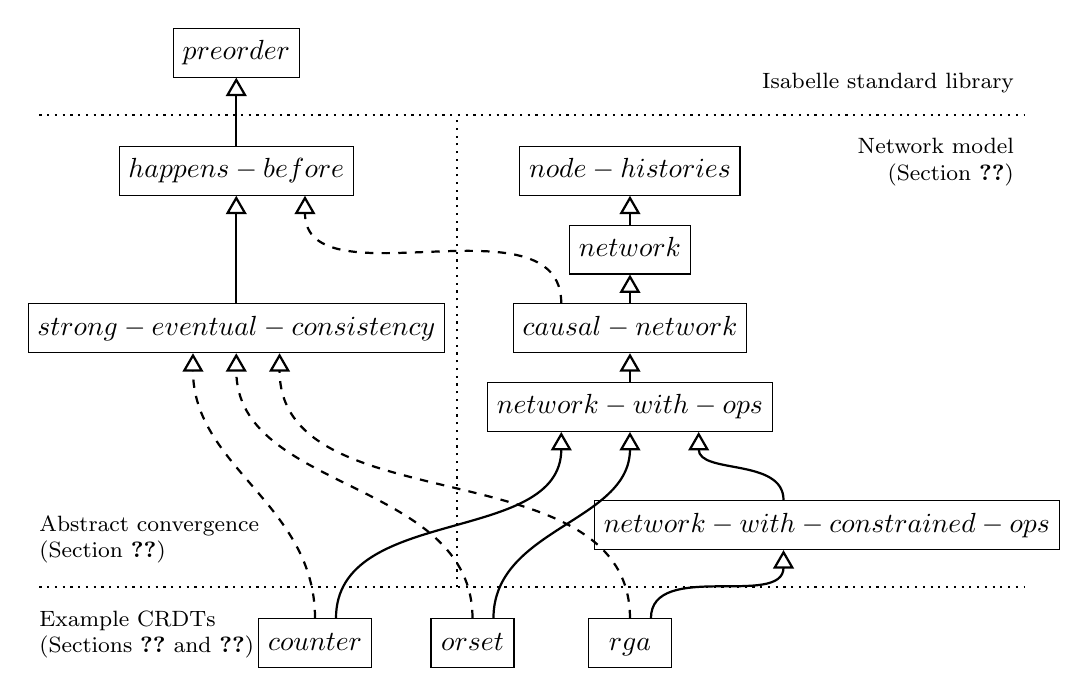
\begin{tikzpicture}[auto,scale=1.0]

\tikzstyle{locale}=[draw,anchor=base,minimum width=30pt,text height=8pt,text depth=3pt]

\node (preorder) at (0,7.5) [locale] {$\isa{preorder}$};
\node (hb)       at (0,6)   [locale] {$\isa{happens-before}$};
\node (sec)      at (0,4)   [locale] {$\isa{strong-eventual-consistency}$};
\node (hist)     at (5,6)   [locale] {$\isa{node-histories}$};
\node (network)  at (5,5)   [locale] {$\isa{network}$};
\node (causal)   at (5,4)   [locale] {$\isa{causal-network}$};
\node (netops)   at (5,3)   [locale] {$\isa{network-with-ops}$};
\node (netops2)  at (7.5,1.5) [locale] {$\isa{network-with-constrained-ops}$};
\node (counter)  at (1,0)   [locale] {$\isa{counter}$};
\node (orset)    at (3,0)   [locale] {$\isa{orset}$};
\node (rga)      at (5,0)   [locale] {$\isa{rga}$};

\begin{scope}[thick,dotted]
    \path [draw] (-2.5,6.8) -- ( 10,6.8);
    \path [draw] (-2.5,0.8) -- ( 10,0.8);
    \path [draw] ( 2.8,0.8) -- (2.8,6.8);
\end{scope}

\begin{scope}[left,text width=5cm,text ragged left,font=\footnotesize]
    \node at (10, 7.2) {Isabelle standard library};
    \node at (10, 6.2) {Network model\\(Section \ref{sect.network})};
\end{scope}
\begin{scope}[text width=5cm,font=\footnotesize]
    \node at (0, 1.4) {Abstract convergence\\(Section \ref{sect.abstract.convergence})};
    \node at (0, 0.2) {Example CRDTs\\(Sections \ref{sect.rga} and \ref{sect.simple.crdts})};
\end{scope}

\begin{scope}[>=open triangle 60]
    \tikzstyle{every path}=[thick,->]
    \draw (hb) to (preorder);
    \draw (sec) to (hb);
    \draw (network) to (hist);
    \draw (causal) to (network);
    \draw (netops) to (causal);
    \draw (node cs:name=netops2,angle=150) to [out=90,in=270] (node cs:name=netops, angle=340);
    \draw (node cs:name=counter,angle=50)  to [out=90,in=270] (node cs:name=netops, angle=200);
    \draw (node cs:name=orset,  angle=50)  to [out=90,in=270] (node cs:name=netops, angle=270);
    \draw (node cs:name=rga,    angle=50)  to [out=90,in=270] (node cs:name=netops2,angle=210);
    \tikzstyle{every path}=[thick,dashed,->]
    \draw (node cs:name=causal, angle=160) to [out=90,in=270] (node cs:name=hb, angle=340);
    \draw (node cs:name=counter,angle=90)  to [out=90,in=270] (node cs:name=sec,angle=210);
    \draw (node cs:name=orset,  angle=90)  to [out=90,in=270] (node cs:name=sec,angle=270);
    \draw (node cs:name=rga,    angle=90)  to [out=90,in=270] (node cs:name=sec,angle=330);
\end{scope}
\end{tikzpicture}

\caption{The main locales (modules) of our proof, and the relationships between them.
Solid arrows indicate a more specialised locale that extends a more general locale (like subclassing in OOP).
Dashed arrows indicate a sublocale that satisfies the assumptions of the superlocale (like implementing an interface in OOP).
}\label{fig.proof.structure}
\end{figure}

By lines of code, more than half of our proof is used to construct a general-purpose model of consistency in distributed systems, described in Section~\ref{sect.abstract.convergence}, and an axiomatic model of a computer network, described in Section~\ref{sect.network}, with both modules independent of any particular replication algorithm.
The remainder describes a formalisation of three CRDTs and their proofs of correctness, described in Sections~\ref{sect.rga} and~\ref{sect.simple.crdts}.
By keeping the general-purpose modules abstract and implementation-independent, we construct a reusable library of specifications and theorems.

We describe our formalisation of strong eventual consistency in Section~\ref{sect.abstract.convergence}.
In particular, we define what we mean by convergence, and prove an \emph{abstract convergence theorem}, which shows that the state of nodes converges if concurrent operations commute.
We are able to prove this fact without mentioning networks or any particular CRDT, but merely by reasoning about the ordering and properties of operations.
This definition constitutes an abstract specification of what we mean by strong eventual consistency.

In Section~\ref{sect.network} we describe an axiomatic model of asynchronous networks.
The definition of the network is important because it allows us to prove that the desired properties hold in \emph{all} possible network behaviours, and that we are not making any dangerous assumptions that might be violated---an aspect that has dogged previous verification efforts for related algorithms (see Section~\ref{sect.related.verification}).
The network is the only part of our proof in which we make any axiomatic assumptions, and we show in Section~\ref{sect.network} that our assumptions are realistic, reflecting both standard conventions for modelling distributed systems, and the practical realities of network protocols today.
We then prove that our network satisfies the ordering properties required by the abstract convergence theorem of Section~\ref{sect.abstract.convergence}, and thus deduce a convergence theorem for our network model.

We use the general-purpose theorems and definitions from Sections~\ref{sect.abstract.convergence} and~\ref{sect.network} to prove the strong eventual consistency properties of concrete algorithms.
In Section~\ref{sect.rga} we describe our formalisation of the Replicated Growable Array (RGA), a CRDT for ordered lists.
We first show how to implement the RGA's insert and delete operations, with proofs that each operation commutes with itself, and that all operations commute with each other.
Insertion and deletion only commute under various conditions, so we prove that these conditions are satisfied in all possible network behaviours, and thus we obtain a concrete convergence theorem for our RGA implementation.
Next, in Section~\ref{sect.simple.crdts}, we demonstrate the generality of our proof framework with definitions of two simple CRDTs: a Counter and an Observed-Remove Set.
%We show that with the previously established tooling in place, it is very easy to prove that these algorithms implement the abstract specification of strong eventual consistency.

As illustrated in Figure~\ref{fig.proof.structure}, the $\isa{counter}$, $\isa{orset}$, and $\isa{rga}$ locales can use the definitions and lemmas of the network model because they extend that model.
We then prove that all three locales satisfy the abstract specification $\isa{strong-eventual-consistency}$, and therefore show that these algorithms provide strong eventual consistency.

\section{Formalising system models using Isabelle}
\label{sect.high-level.proof.strategy}

All of our proofs are checked with the Isabelle/HOL proof assistant~\cite{DBLP:conf/tphol/WenzelPN08}, which we now briefly introduce so that the reader can easily follow our work.
A more detailed introduction is provided by standard tutorial material~\cite{DBLP:books/sp/NipkowK14}.

In this section, we provide a high-level overview of our proof strategy, so readers can more easily understand our Isabelle development.

In Section~\ref{sect.abstract.convergence} we present an `abstract convergence theorem' which does not mention networks, nor does it mention any machinery tied to any one particular CRDT implementation. 
Rather, the theorem statement is phrased in terms of purely abstract `events', and functions that lift events into abstract `state formers'.
As a result, the theorem may be viewed purely as a property of preorders, or alternatively as a `distillation' of the notion of SEC convergence, which gives sufficient conditions for convergence in this setting.

In Section~\ref{sect.network} we provide an axiomatic model of causal asynchronous networks, built around a broadcast-deliver event model.
We develop a relation---\emph{happens before}---which captures the notion of `causality' within this network---and is a preorder.
The abstract convergence theorem of Section~\ref{sect.abstract.convergence} therefore applies, and we `compose' this theorem with our network model, to obtain a convergence theorem for our network.

Note that everything mentioned until this point is completely generic---we are not tied to any CRDT implementation.
However, we may now use our abstract convergence theorems to prove concrete convergence theorems for given CRDT implementations.

We present a concrete example in Section~\ref{sect.rga}: a mechanisation of the Replicated Growable Array (RGA).
We first implement the RGA's insert and delete operations, with proofs that each operation commutes with itself, and all operations commute with each other.
Insertion and deletion only commute under various conditions, which are reflected in a constraining of all possible network behaviours to only those that guarantee that the RGA CRDT remains `well behaved'.
This constraining can be viewed as an associated `protocol' for the RGA, detailing valid modes of usage of the data type.
The constrained network provides the right conditions under which all operations commute with each other, and as a corollary of our abstract convergence theorem, we obtain a concrete convergence theorem for our RGA implementation in a constrained network.


\subsection{An overview of Isabelle}
\label{subsect.an.overview.of.isabelle}

Isabelle/HOL is a logic with a strict, polymorphic type system resembling that of mainstream functional programming languages.
\emph{Function types} are written $\tau_1 \Rightarrow \tau_2$, and are inhabited by \emph{total} functions, mapping elements of $\tau_1$ to elements of $\tau_2$.
We write $\tau_1 \times \tau_2$ for the \emph{product type} of $\tau_1$ and $\tau_2$, inhabited by pairs of elements of type $\tau_1$ and $\tau_2$, respectively.
In a similar fashion to Standard ML and OCaml, but differing from Haskell, \emph{type operators} are applied to arguments in reverse order, and therefore write $\tau\ \isa{list}$ and $\tau\ \isa{set}$ for the type of lists of elements of type $\tau$, and the type of mathematical (i.e. potentially infinite) sets of type $\tau$, respectively.
Type variable are written in lowercase, and preceded with a prime: ${\isacharprime}a \Rightarrow {\isacharprime}a$ denotes the type of a polymorphic identity function, for example.
\emph{Tagged union} types are introduced with the $\isacommand{datatype}$ keyword, with constructors of these types written with an initial upper case letter.

In Isabelle/HOL's term language we write $\isa{t} \isa{::} \tau$ for a \emph{type ascription}, constraining the type of the term $\isa{t}$ to the type $\tau$.
We write $\lambda{x}. t$ for an anonymous function mapping an argument $\isa{x}$ to $\isa{t(x)}$, and write the application of term $\isa{t}$ with function type to an argument $\isa{u}$ as $\isa{t\ u}$, as usual.
Terms of list type are introduced using one of two constructors: $\isa{[]}$, or `nil', standing for the empty list, and infix $\isa{\#}$, or `cons', which prepends an element to an existing list.
We use $[t_1, \ldots, t_n]$ as syntactic sugar for a list literal, which is desugared into a series of cons applications.
We write $\{\}$ for the empty set, and use usual mathematical notation for set union, disjunction, membership tests, and so on: $\isa{t} \cup \isa{u}$, $\isa{t} \cap \isa{u}$, and $\isa{x} \in \isa{t}$.

Terms with type $\isa{bool}$ are called \emph{formulae}, writing $\isa{True}$ and $\isa{False}$ for the logical truthity and falsity constants, respectively.
We write $\isa{t} \longrightarrow \isa{u}$, $\isa{t} \wedge \isa{u}$, and $\isa{t} \vee \isa{u}$ for material implication, conjunction, and disjunction, respectively, between formulae, and write $\neg t$ for the negation of a formula.
Isabelle/HOL's equality constant is polymorphic: we write $t = u$ for an assertion of equality between two terms of the same type.
We write $\forall{x}.t$ and $\exists{x}.t$ for universal and existential quantification---and write $\forall{x{\in}t}.u$ and $\exists{x{\in}t}.u$ for their bounded forms, restricted to members of a set $\isa{t}$.
An alternative implication arrow $\isa{t} \Longrightarrow \isa{u}$ may sometimes be used, and is in fact required by Isabelle in certain contexts---an artefact of Isabelle's status as a logical framework.
This arrow can safely be read as a standard implication arrow with little loss of understanding.

New non-recursive definitions are entered into Isabelle's global context via the $\mathbf{definition}$ keyword.
Recursive functions are entered via the $\mathbf{fun}$ keyword, with functions being defined piecewise by pattern matching on inputs with a series of equations.
All function are total, and therefore recursive functions must be provably terminating, in that they recurse on arguments that are `smaller' with respect to a well-founded relation.
All termination proofs in this work are generated automatically by Isabelle itself.

Inductive relations are introduced with the $\mathbf{inductive}$ keyword.
An inductive relation definition of the form
\vspace{0.375em}
\begin{isabellebody}
\ \ \ \ \ \ \ \ \isacommand{inductive} foo\ {\isacharcolon}{\isacharcolon}\ {\isachardoublequoteopen}nat\ list\ {\isasymRightarrow}\ bool{\isachardoublequoteclose}\ \isakeyword{where}\isanewline
\ \ \ \ \ \ \ \ \ \ {\isachardoublequoteopen}foo\ {\isacharbrackleft}{\isacharbrackright}{\isachardoublequoteclose}\ {\isacharbar}\isanewline
\ \ \ \ \ \ \ \ \ \ {\isachardoublequoteopen}{\isasymlbrakk}\ foo\ xs\ {\isasymrbrakk}\ {\isasymLongrightarrow}\ foo {\isacharparenleft}5\#xs{\isacharparenright}{\isachardoublequoteclose}
\end{isabellebody}
\vspace{0.375em}
\noindent
introduces a new constant $\isa{foo}$ of type $\isa{nat list} \Rightarrow \isa{bool}$.
The two clauses in the body of the definition enumerate the conditions under which $\isa{foo}\ \isa{xs}$ is true, for arbitrary $\isa{xs}$.
The definition above states that $\isa{foo}$ is true at the empty list, or given a proof that $\isa{foo}\ \isa{xs}$ is true for some $\isa{xs}$, then $\isa{foo}\ (5\#\isa{xs})$ is true, also.
Further, $\isa{foo}\ \isa{xs}$ is true in no other circumstances---$\isa{foo}$ is the \emph{smallest} relation closed under the rules defining it.
In short, the clauses defining $\isa{foo}$ above state that $\isa{foo}\ \isa{xs}$ holds exactly in the case where $\isa{xs}$ is a (potentially empty) list containing only repeated copies of the natural number $5$.

Lemmas, theorems, and corollaries can be asserted using the $\isacommand{lemma}$, $\isacommand{theorem}$, and $\isacommand{corollary}$ keywords, respectively.
There is no semantic difference between these keywords in Isabelle.
A theorem statement of the form
\vspace{0.375em}
\begin{isabellebody}
\ \ \ \ \ \ \ \ \isacommand{theorem} goo{\isacharcolon}\isanewline
\ \ \ \ \ \ \ \ \ \ \isakeyword{assumes}\ foo\ xs \isakeyword{and}\ foo\ ys \isanewline
\ \ \ \ \ \ \ \ \ \ \isakeyword{shows}\ foo (xs \isacharat ys)
\end{isabellebody}
\vspace{0.375em}
\noindent
produces a proof obligation, wherein the user is tasked with proving $\isa{foo} (xs \isacharat ys)$ under the two assumptions $\isa{foo}\ xs$ and $\isa{foo}\ ys$, where $xs \isacharat ys$ is list append.
An optional name, here $\isa{goo}$, is assigned to the theorem, so that it may be referenced in later proofs.

Lastly, we use \emph{locales}---or local theory environments~\cite{DBLP:conf/tphol/KammullerWP99,DBLP:conf/types/HaftmannW08}---extensively throughout our development to structure the proof.
A declaration of the form
\vspace{0.375em}
\begin{isabellebody}
\ \ \ \ \ \ \ \ \isacommand{locale} hoo = \isanewline
\ \ \ \ \ \ \ \ \ \ \isakeyword{fixes}\ f\ {\isacharcolon}{\isacharcolon}\ {\isachardoublequoteopen}{\isacharprime}a\ {\isasymRightarrow}\ {\isacharprime}a{\isachardoublequoteclose}\isanewline
\ \ \ \ \ \ \ \ \ \ \isakeyword{assumes} {\isachardoublequoteopen}f\ x = x{\isachardoublequoteclose}
\end{isabellebody}
\vspace{0.375em}
\noindent
introduces a local theory, with a fixed, typed constant $\isa{f}$, and an associated law that states that $\isa{f}$ is the identity function.
Functions and constants may now be defined, and theorems conjectured and proved, within the context of the $\isa{hoo}$ theory.
This is indicated syntactically by writing $(\isacommand{in}\ hoo)$ before the name of the constant being defined, or the theorem being conjectured, at the point of definition or conjecture.
Any function, constant, or theorem, marked in this way may make reference to $\isa{f}$, or the fact that $\isa{f}\ \isa{x} = \isa{x}$ for all $\isa{x}$.
\emph{Interpreting} a local theory---such as $\isa{hoo}$ above---involves providing a concrete implementation of $\isa{f}$ coupled with a proof that the concrete implementation satisfies the associated law.
Once interpreted, all functions, definitions, and theorems made within the $\isa{hoo}$ local theory become available to use for that concrete implementation.

\section{Abstract convergence}
\label{sect.abstract.convergence}

Strong eventual consistency requires \emph{convergence} of all copies of shared state stored on nodes in the distributed system.
It guarantees that whenever two nodes have received the same set of updates to shared state---possibly in a different order---their view of the shared state is always identical.
This definition constrains the values that read operations may return at any time, making it a stronger property than eventual consistency.
By accessing only their local copy of the shared state, nodes can execute read and write operations without waiting for network communication.
Nodes exchange updates asynchronously when a network connection is available.  

We now use Isabelle to formalise the notion of strong eventual consistency.
In this section we do not make any assumptions about networks, data structures, or conflict resolution algorithms; instead, we use an abstract model of operations that may be reordered, and we reason about the properties that those operations must satisfy.
We then provide concrete implementations of that abstract model in later sections.

\subsection{The happens-before relation and causality}\label{sect.happens.before}

The simplest way of achieving convergence is to require all operations to be commutative, but this definition is too strong to be useful for many datatypes.
For example, in a list data structure, an element may first be added and then subsequently removed again.
Although it is possible to make such additions and removals unconditionally commutative, doing so yields counterintuitive semantics \cite{Bieniusa:2012wu,Bieniusa:2012gt}.
Instead, a better approach is to require only \emph{concurrent} operations to commute with each other.
Two operations are concurrent if neither ``knew about'' the other at the time when they were generated.
If one operation happened before another---for example, if the removal of an element from a set knew about the prior addition of that element from the set---then it is reasonable to assume that all nodes will apply the operations in that order (first the addition, then the removal).

The \emph{happens-before} relation, as introduced by \citet{Lamport:1978jq}, captures such causal dependencies between operations.
It can be defined in terms of sending and receiving messages on a network, and we give such a definition in Section~\ref{sect.network}.
However, for now, we keep it abstract, writing $\isa{x} \prec \isa{y}$ to indicate that operation $\isa{x}$ happened before $\isa{y}$, where $\prec$ is a predicate of type $\isacharprime\isa{oper} \mathbin{\isasymRightarrow} \isacharprime\isa{oper} \mathbin{\isasymRightarrow} \isa{bool}$.
In words, $\prec$ can be applied to two operations of some abstract type $\isacharprime\isa{oper}$, returning either $\isa{True}$ or $\isa{False}$.%
\footnote{Note that in the distributed systems literature it is conventional to write the happens-before relation as $\isa{x} \rightarrow \isa{y}$, but we reserve the arrow operator to denote logical implication.}
Our only restriction on the happens-before relation $\prec$ is that it must be a \emph{strict partial order}, that is, it must be irreflexive and transitive, which implies that it is also antisymmetric.
We say that two operations $x$ and $y$ are \emph{concurrent}, written $x \mathbin{\isasymparallel} y$, whenever one does not happen before the other:
$\neg (\isa{x} \prec \isa{y})$ and $\neg (\isa{y} \prec \isa{x})$.
Thus, given any two operations $\isa{x}$ and $\isa{y}$, there are three mutually exclusive ways in which they can be related: either $\isa{x} \prec \isa{y}$, or $\isa{y} \prec \isa{x}$, or $\isa{x} \mathbin{\isasymparallel} \isa{y}$.

As discussed above, the purpose of the happens-before relation is to require that some operations must be applied in a particular order, while allowing concurrent operations to be reordered with respect to each other.
We assume that each node applies operations in some sequential order (a standard assumption for distributed algorithms), and so we can model the execution history of a node as a list of operations.
We can then inductively define a list of operations as being \emph{consistent with the happens-before relation}, or simply \emph{hb-consistent}, as follows:
\vspace{0.35em}
\begin{isabellebody}
\ \ \ \ \ \ \ \ \isacommand{inductive} hb{\isacharunderscore}consistent\ {\isacharcolon}{\isacharcolon}\ {\isachardoublequoteopen}{\isacharprime}oper\ list\ {\isasymRightarrow}\ bool{\isachardoublequoteclose}\ \isakeyword{where}\isanewline
\ \ \ \ \ \ \ \ \ \ {\isachardoublequoteopen}hb{\isacharunderscore}consistent\ {\isacharbrackleft}{\isacharbrackright}{\isachardoublequoteclose}\ {\isacharbar}\isanewline
\ \ \ \ \ \ \ \ \ \ {\isachardoublequoteopen}{\isasymlbrakk}\ hb{\isacharunderscore}consistent\ xs{\isacharsemicolon}\ {\isasymforall}x\ {\isasymin}\ set\ xs{\isachardot}\ {\isasymnot}\ y\ {\isasymprec}\ x\ {\isasymrbrakk}\ {\isasymLongrightarrow}\ hb{\isacharunderscore}consistent\ {\isacharparenleft}xs\ {\isacharat}\ {\isacharbrackleft}y{\isacharbrackright}{\isacharparenright}{\isachardoublequoteclose}
\end{isabellebody}
\vspace{0.35em}
In words: the empty list is hb-consistent; furthermore, given an hb-consistent list $\isa{xs}$, we can append an operation $\isa{y}$ to the end of the list to obtain another hb-consistent list, provided that $\isa{y}$ does not happen-before any existing operation $\isa{x}$ in $\isa{xs}$. As a result, whenever two operations $\isa{x}$ and $\isa{y}$ appear in a hb-consistent list, and $\isa{x}\prec\isa{y}$, then $\isa{x}$ must appear before $\isa{y}$ in the list. However, if $\isa{x}\mathbin{\isasymparallel}\isa{y}$, the operations can appear in the list in either order.

\subsection{Interpretation of operations}\label{sect.ops.interpretation}

We describe the state of a node using an abstract type variable $\isacharprime\isa{state}$.
To model state changes, we assume the existence of an \emph{interpretation} function of type $\isa{interp} \mathbin{\isacharcolon\isacharcolon} \isacharprime\isa{oper} \mathbin{\isasymRightarrow} \isacharprime\isa{state} \mathbin{\isasymRightarrow} \isacharprime\isa{state}\ \isa{option}$, which lifts an operation into a \emph{state transformer}---a function that either maps an old state to a new state, or fails by returning $\isa{None}$.
If $\isa{x}$ is an operation, we also write $\langle\isa{x}\rangle$ for the state transformer obtained by applying $\isa{x}$ to the interpretation function.

Concretely, these definitions are captured in Isabelle with the following locale declaration:
\vspace{0.35em}
\begin{isabellebody}
\ \ \ \ \ \ \ \ \isacommand{locale} happens{\isacharunderscore}before\ {\isacharequal}\ preorder\ hb{\isacharunderscore}weak\ hb\isanewline
\ \ \ \ \ \ \ \ \ \ \isakeyword{for}\ hb{\isacharunderscore}weak\ {\isacharcolon}{\isacharcolon}\ {\isachardoublequoteopen}{\isacharprime}oper\ {\isasymRightarrow}\ {\isacharprime}oper\ {\isasymRightarrow}\ bool{\isachardoublequoteclose}\ \ {\isacharparenleft}\isakeyword{infix}\ {\isachardoublequoteopen}{\isasympreceq}{\isachardoublequoteclose}\ {\isadigit{5}}{\isadigit{0}}{\isacharparenright}\ \isakeyword{and}\ hb\ {\isacharcolon}{\isacharcolon}\ {\isachardoublequoteopen}{\isacharprime}oper\ {\isasymRightarrow}\ {\isacharprime}oper\ {\isasymRightarrow}\ bool{\isachardoublequoteclose}\ \ {\isacharparenleft}\isakeyword{infix}\ {\isachardoublequoteopen}{\isasymprec}{\isachardoublequoteclose}\ {\isadigit{5}}{\isadigit{0}}{\isacharparenright}\ {\isacharplus}\isanewline
\ \ \ \ \ \ \ \ \ \ \isakeyword{fixes}\ interp\ {\isacharcolon}{\isacharcolon}\ {\isachardoublequoteopen}{\isacharprime}oper\ {\isasymRightarrow}\ {\isacharprime}state\ {\isasymRightarrow}\ {\isacharprime}state\ option{\isachardoublequoteclose}\ {\isacharparenleft}{\isachardoublequoteopen}{\isasymlangle}{\isacharunderscore}{\isasymrangle}{\isachardoublequoteclose}\ {\isacharbrackleft}{\isadigit{0}}{\isacharbrackright}\ {\isadigit{1}}{\isadigit{0}}{\isadigit{0}}{\isadigit{0}}{\isacharparenright}
\end{isabellebody}
\vspace{0.35em}
The $\isa{happens-before}$ locale extends the $\isa{preorder}$ locale, which is part of Isabelle's standard library and includes various useful lemmas.
It fixes two constants: a preorder that we call $\isa{hb-weak}$ or $\preceq$, and a strict partial order that we call $\isa{hb}$ or $\prec$.
We are only interested in the strict partial order, so we define $\isa{hb-weak}$ as $\isa{x}\preceq\isa{y} \equiv \isa{x}\prec\isa{y} \vee \isa{x}=\isa{y}$, and otherwise ignore it.

Moreover, the locale fixes the interpretation function $\isa{interp}$ as described above, which means that we assume the existence of a function with the given type signature without specifying an implementation.
The code in parentheses defines the mixfix operators $\preceq$, $\prec$, and $\langle\isa{x}\rangle$ for notational convenience.

Given two operations $\isa{x}$ and $\isa{y}$, we can now define the composition of state transformers: we write $\langle\isa{x}\rangle \mathbin{\isasymrhd} \langle\isa{y}\rangle$ to denote the state transformer that first applies the effect of $\isa{x}$ to some state, and then applies the effect of $\isa{y}$ to the result.
If either $\langle\isa{x}\rangle$ or $\langle\isa{y}\rangle$ fails, the combined state transformer also fails.
The operator $\isasymrhd$ is a specialised form of the \emph{Kleisli arrow composition}, which we define as:
\vspace{0.35em}
\begin{isabellebody}
\ \ \ \ \ \ \ \ \isacommand{definition} kleisli\ {\isacharcolon}{\isacharcolon}\ {\isachardoublequoteopen}{\isacharparenleft}{\isacharprime}a\ {\isasymRightarrow}\ {\isacharprime}a\ option{\isacharparenright}\ {\isasymRightarrow}\ {\isacharparenleft}{\isacharprime}a\ {\isasymRightarrow}\ {\isacharprime}a\ option{\isacharparenright}\ {\isasymRightarrow}\ {\isacharparenleft}{\isacharprime}a\ {\isasymRightarrow}\ {\isacharprime}a\ option{\isacharparenright}{\isachardoublequoteclose}\ {\isacharparenleft}\isakeyword{infixr}\ {\isachardoublequoteopen}{\isasymrhd}{\isachardoublequoteclose}\ {\isadigit{6}}{\isadigit{5}}{\isacharparenright}\ \isakeyword{where}\isanewline
\ \ \ \ \ \ \ \ \ \ {\isachardoublequoteopen}f\ {\isasymrhd}\ g\ {\isasymequiv}\ {\isasymlambda}x{\isachardot}\ f\ x\ {\isasymbind}\ {\isacharparenleft}{\isasymlambda}y{\isachardot}\ g\ y{\isacharparenright}{\isachardoublequoteclose}
\end{isabellebody}
\vspace{0.35em}
Here, $\isasymbind$ is the \emph{monadic bind} operation, defined on the option type that we are using to implement partial functions.
We can now define a function $\isa{apply-operations}$ that composes an arbitrary list of operations into a state transformer.
We first map $\isa{interp}$ across the list to obtain a state transformer for each operation, and then collectively compose them using the Kleisli arrow composition combinator:
\vspace{0.35em}
\begin{isabellebody}
\ \ \ \ \ \ \ \ \isacommand{definition} apply{\isacharunderscore}operations\ {\isacharcolon}{\isacharcolon}\ {\isachardoublequoteopen}{\isacharprime}oper\ list\ {\isasymRightarrow}\ {\isacharprime}state\ {\isasymRightarrow}\ {\isacharprime}state\ option{\isachardoublequoteclose}\ \isakeyword{where}\isanewline
\ \ \ \ \ \ \ \ \ \ {\isachardoublequoteopen}apply{\isacharunderscore}operations\ es\ {\isasymequiv}\ foldl\ {\isacharparenleft}op\ {\isasymrhd}{\isacharparenright}\ Some\ {\isacharparenleft}map\ interp\ es{\isacharparenright}{\isachardoublequoteclose}
\end{isabellebody}
\vspace{0.35em}
The result is a state transformer that applies the interpretation of each of the operations in the list, in left-to-right order, to some initial state.
If any of the operations fails, the entire composition returns $\isa{None}$.

\subsection{Commutativity and convergence}\label{sect.ops.commute}

We say that two operations $\isa{x}$ and $\isa{y}$ \emph{commute} whenever $\langle\isa{x}\rangle \mathbin{\isasymrhd} \langle\isa{y}\rangle = \langle\isa{y}\rangle \mathbin{\isasymrhd} \langle\isa{x}\rangle$, i.e. when we can swap the order of the composition of their interpretations without changing the resulting state transformer.
For our purposes, requiring that this property holds for \emph{all} pairs of operations is too strong.
Rather, the commutation property is only required to hold for operations that are concurrent, as captured in the next definition:
\vspace{0.35em}
\begin{isabellebody}
\ \ \ \ \ \ \ \ \isacommand{definition} concurrent{\isacharunderscore}ops{\isacharunderscore}commute\ {\isacharcolon}{\isacharcolon}\ {\isachardoublequoteopen}{\isacharprime}oper\ list\ {\isasymRightarrow}\ bool{\isachardoublequoteclose}\ \isakeyword{where}\isanewline
\ \ \ \ \ \ \ \ \ \ {\isachardoublequoteopen}concurrent{\isacharunderscore}ops{\isacharunderscore}commute\ xs\ {\isasymequiv} {\isasymforall}x\ y{\isachardot}\ {\isacharbraceleft}x{\isacharcomma}\ y{\isacharbraceright}\ {\isasymsubseteq}\ set\ xs\ {\isasymlongrightarrow}\ x\ {\isasymparallel}\ y\ {\isasymlongrightarrow}\ {\isasymlangle}x{\isasymrangle}{\isasymrhd}{\isasymlangle}y{\isasymrangle}\ {\isacharequal}\ {\isasymlangle}y{\isasymrangle}{\isasymrhd}{\isasymlangle}x{\isasymrangle}{\isachardoublequoteclose}
\end{isabellebody}
\vspace{0.35em}
Given this definition, we can now state and prove our main theorem, $\isa{convergence}$.
This theorem states that two hb-consistent lists of distinct operations, which are permutations of each other and in which concurrent operations commute, have the same interpretation:
\vspace{0.35em}
\begin{isabellebody}
\ \ \ \ \ \ \ \ \isacommand{theorem} convergence{\isacharcolon}\isanewline
\ \ \ \ \ \ \ \ \ \ \isakeyword{assumes}\ {\isachardoublequoteopen}set\ xs\ {\isacharequal}\ set\ ys{\isachardoublequoteclose}\ \isakeyword{and}\ {\isachardoublequoteopen}concurrent{\isacharunderscore}ops{\isacharunderscore}commute\ xs{\isachardoublequoteclose}\ \isakeyword{and}\ {\isachardoublequoteopen}concurrent{\isacharunderscore}ops{\isacharunderscore}commute\ ys{\isachardoublequoteclose}\isanewline
\ \ \ \ \ \ \ \ \ \ \ \ \ \ \ \ \isakeyword{and}\ {\isachardoublequoteopen}distinct\ xs{\isachardoublequoteclose}\ \isakeyword{and}\ {\isachardoublequoteopen}distinct\ ys{\isachardoublequoteclose}\ \isakeyword{and}\ {\isachardoublequoteopen}hb{\isacharunderscore}consistent\ xs{\isachardoublequoteclose}\ \isakeyword{and}\ {\isachardoublequoteopen}hb{\isacharunderscore}consistent\ ys{\isachardoublequoteclose}\isanewline
\ \ \ \ \ \ \ \ \ \ \isakeyword{shows}\ {\isachardoublequoteopen}apply{\isacharunderscore}operations\ xs\ {\isacharequal}\ apply{\isacharunderscore}operations\ ys{\isachardoublequoteclose}
\end{isabellebody}
\vspace{0.35em}
\noindent
A fully mechanised proof of this theorem can be found in the supplementary material of this paper.
Although this theorem may seem ``obvious'' at first glance---commutativity allows the operation order to be permuted---it is more subtle than it seems.
The difficulty arises because operations may succeed when applied to some state, but fail when applied to another state (for example, deleting an element that does not exist in the state).
We find it interesting that it is nevertheless sufficient for the definition of $\isa{concurrent-ops-commute}$ to be expressed only in terms of the Kleisli arrow composition, and without explicitly referring to the state.

\subsection{Formalising Strong Eventual Consistency}\label{sect.abstract.sec.spec}

Besides convergence, another required property of SEC is \emph{progress}: if a valid operation was issued on one node, then applying that operation on other nodes must also succeed---that is, the execution must not become stuck in an error state.
Although the type signature of the interpretation function allows operations to fail, we need to prove that in all $\isa{hb-consistent}$ executions such failure never actually occurs.
We capture the combined requirements of convergence and progress in the $\isa{strong-eventual-consistency}$ locale, which extends $\isa{happens-before}$:
\vspace{0.35em}
\begin{isabellebody}
\ \ \ \ \ \ \ \ \isacommand{locale}\ strong{\isacharunderscore}eventual{\isacharunderscore}consistency\ {\isacharequal}\ happens{\isacharunderscore}before\ {\isacharplus}\ \isakeyword{fixes}\ op{\isacharunderscore}history\ {\isacharcolon}{\isacharcolon}\ {\isachardoublequoteopen}{\isacharprime}oper\ list\ {\isasymRightarrow}\ bool{\isachardoublequoteclose}\ \isakeyword{and}\ initial{\isacharunderscore}state\ {\isacharcolon}{\isacharcolon}\ {\isachardoublequoteopen}{\isacharprime}state{\isachardoublequoteclose}\isanewline
\ \ \ \ \ \ \ \ \ \ \isakeyword{assumes}\ causality{\isacharcolon}\ \ \ \ \ {\isachardoublequoteopen}op{\isacharunderscore}history\ xs\ {\isasymLongrightarrow}\ hb{\isacharunderscore}consistent\ xs{\isachardoublequoteclose}\isanewline
\ \ \ \ \ \ \ \ \ \ \ \ \ \ \isakeyword{and}\ distinctness{\isacharcolon}\ \ {\isachardoublequoteopen}op{\isacharunderscore}history\ xs\ {\isasymLongrightarrow}\ distinct\ xs{\isachardoublequoteclose}\isanewline
\ \ \ \ \ \ \ \ \ \ \ \ \ \ \isakeyword{and}\ trunc{\isacharunderscore}history{\isacharcolon}\ {\isachardoublequoteopen}op{\isacharunderscore}history{\isacharparenleft}xs{\isacharat}{\isacharbrackleft}x{\isacharbrackright}{\isacharparenright}\ {\isasymLongrightarrow}\ op{\isacharunderscore}history\ xs{\isachardoublequoteclose}\isanewline
\ \ \ \ \ \ \ \ \ \ \ \ \ \ \isakeyword{and}\ commutativity{\isacharcolon}\ {\isachardoublequoteopen}op{\isacharunderscore}history\ xs\ {\isasymLongrightarrow}\ concurrent{\isacharunderscore}ops{\isacharunderscore}commute\ xs{\isachardoublequoteclose}\isanewline
\ \ \ \ \ \ \ \ \ \ \ \ \ \ \isakeyword{and}\ no{\isacharunderscore}failure{\isacharcolon}\ \ \ \ {\isachardoublequoteopen}op{\isacharunderscore}history{\isacharparenleft}xs{\isacharat}{\isacharbrackleft}x{\isacharbrackright}{\isacharparenright}\ {\isasymLongrightarrow}\ apply{\isacharunderscore}operations\ xs\ initial{\isacharunderscore}state\ {\isacharequal}\ Some\ state\ {\isasymLongrightarrow}\ {\isasymlangle}x{\isasymrangle}\ state\ {\isasymnoteq}\ None{\isachardoublequoteclose}
\end{isabellebody}
\vspace{0.35em}
Here, $\isa{op-history}$ is an abstract predicate describing any valid operation history of some replication algorithm.
This locale serves as a concise summary of the properties that we require in order to achieve SEC, and from these assumptions and the theorem above we easily obtain the two safety properties of SEC as theorems:
\vspace{0.35em}
\begin{isabellebody}
\ \ \ \ \ \ \ \ \isacommand{theorem}\ {\isacharparenleft}\isakeyword{in}\ strong{\isacharunderscore}eventual{\isacharunderscore}consistency{\isacharparenright}\ sec{\isacharunderscore}convergence{\isacharcolon}\isanewline
\ \ \ \ \ \ \ \ \ \ \isakeyword{assumes}\ {\isachardoublequoteopen}set\ xs\ {\isacharequal}\ set\ ys{\isachardoublequoteclose}\ \isakeyword{and}\ {\isachardoublequoteopen}op{\isacharunderscore}history\ xs{\isachardoublequoteclose}\ \isakeyword{and}\ {\isachardoublequoteopen}op{\isacharunderscore}history\ ys{\isachardoublequoteclose}\isanewline
\ \ \ \ \ \ \ \ \ \ \isakeyword{shows}\ \ \ {\isachardoublequoteopen}apply{\isacharunderscore}operations\ xs\ {\isacharequal}\ apply{\isacharunderscore}operations\ ys{\isachardoublequoteclose}
\end{isabellebody}
\vspace{0.35em}
\begin{isabellebody}
\ \ \ \ \ \ \ \ \isacommand{theorem}\ {\isacharparenleft}\isakeyword{in}\ strong{\isacharunderscore}eventual{\isacharunderscore}consistency{\isacharparenright}\ sec{\isacharunderscore}progress{\isacharcolon}\isanewline
\ \ \ \ \ \ \ \ \ \ \isakeyword{assumes}\ {\isachardoublequoteopen}op{\isacharunderscore}history\ xs{\isachardoublequoteclose}\isanewline
\ \ \ \ \ \ \ \ \ \ \isakeyword{shows}\ \ \ {\isachardoublequoteopen}apply{\isacharunderscore}operations\ xs\ initial{\isacharunderscore}state\ {\isasymnoteq}\ None{\isachardoublequoteclose}
\end{isabellebody}
\vspace{0.35em}
Thus, in order to prove SEC for some replication algorithm, we only need to show that the five assumptions of the $\isa{strong-eventual-consistency}$ locale are satisfied.
As we shall see in Section~\ref{sect.network}, the first three assumptions are satisfied by our network model, and do not require any algorithm-specific proofs.
For individual algorithms we only need to prove the $\isa{commutativity}$ and $\isa{no-failure}$ properties, and we show how to do this in Sections~\ref{sect.rga} and~\ref{sect.simple.crdts}.

\section{An axiomatic network model}
\label{sect.network}

In this section, we provide a formal definition of an asynchronous unreliable causal broadcast network, giving us a realistic setting in which we can embed various replication algorithms, and prove that they guarantee strong eventual consistency in all possible behaviours of the network.
Our network model is defined using only six axioms, all of which are standard assumptions in the modelling of distributed systems, and which are satisfied by many systems in practice.
All theorems in this paper are derived from those axioms; in particular, we show that the causal delivery abstraction satisfies the strict partial ordering assumption of $\isa{hb-consistent}$ (Section~\ref{sect.happens.before}), allowing us to use the $\isa{convergence}$ theorem (Section~\ref{sect.ops.commute}) in locales that extend the network.

%TODO Martin to check that he is happy with the rest of this intro. Have we stated informally why we want to model an asynchronous unreliable causal broadcast network and what this means?
We start by assuming that all communication between nodes are sent as messages via the network and that these messages may be delayed, reordered, or lost entirely---an assumption that matches the behaviour of many networks in practice~\cite{Bailis:2014jx}.
Moreover, nodes or network links may fail at any time, and the non-faulty parts of the system need
to continue working in spite of such partial failures.

As motivated in the Introduction, we do not wish to rely on a central server.
Rather, we aim to support scenarios in which subsets of nodes can communicate with each other, but some are disconnected (\emph{partitioned}) from others.
It is possible to provide totally ordered delivery without a central server and thus obtain strong consistency; this abstraction is known as \emph{total order broadcast} or \emph{atomic broadcast} \cite{Cachin:2011wt,Defago:2004ji}.
Unfortunately, it is expensive: it requires a quorum of nodes (typically a majority) to be reachable in order to make progress \cite{Chandra:1996cp}.
This is not an assumption we wish to make since, when nodes represent laptops or smartphones, it is likely that less than a majority of devices are online at any one time, and so any algorithm for total order broadcast would be stalled.
For example, consider some data shared between two users, each of whom has two devices. 
Each user may want to synchronise the data between their two devices using a local wireless link, even if they are temporarily disconnected from the internet, and re-synchronise with the other user when they are next online. 
In this scenario, strong consistency across both users could only be achieved by preventing users from making any offline updates; if updates are allowed, weaker consistency is inevitable \cite{Attiya:2015dm,Davidson:1985hv}.

We therefore use an \emph{asynchronous} network model, which means that we make no timing assumptions: messages sent over the network may suffer unbounded delays before they are delivered, or they may never arrive at all. 
Nodes may pause their execution for unbounded periods of time, or fail permanently \cite{Cachin:2011wt}. 
If a user makes updates while offline, and the device re-synchronises when it is next online, we can simply model that interaction as very large network delay.
Moreover, if network interruptions between nodes last only for a finite time, every update can be eventually delivered to every non-failed node by re-sending messages until they arrive.
%Thus, all non-failed nodes will eventually deliver the same set of updates (although perhaps in a different order), and
%so strong eventual consistency will ensure that they all converge to an equivalent state. 
We can therefore assume that the network is \emph{unreliable}.
If nodes are partitioned from each other forever, they will not converge, but that is the case for any replication algorithm, since the network is assumed to be the only communication channel.
In such cases we assume that the node has failed.

%Although most practical systems have fairly low network delay and fairly brief execution pauses most of the time, the asynchronous model is a useful lower bound for the assumptions that a distributed algorithm may make. 
%Any algorithm that is proved correct under the assumptions of the asynchronous model is also guaranteed to be correct in a system that provides stronger guarantees, for example around timing and reliability.

\subsection{Modelling a distributed system}

We model a distributed system as an unbounded number of communicating nodes.
We do not assume anything about the communication pattern of nodes---we assume only that each node is uniquely identified by a natural number, and that the flow of execution at each node consists of a finite, totally ordered sequence of execution steps (events).
We call that sequence of events at node $i$ the \emph{history} of that node.
For convenience, we assume that every event or execution step is unique within a node's history; this assumption is standard in the modelling of distributed systems \cite{Cachin:2011wt} and can easily be implemented by attaching a sequence number, timestamp, or other unique identifier to each event.
This system model can be expressed in Isabelle as follows:
\vspace{0.35em}
\begin{isabellebody}
\ \ \ \ \ \ \ \ \isacommand{locale} node{\isacharunderscore}histories\ {\isacharequal}\ \isanewline
\ \ \ \ \ \ \ \ \ \ \isakeyword{fixes}\ history\ {\isacharcolon}{\isacharcolon}\ {\isachardoublequoteopen}nat\ {\isasymRightarrow}\ {\isacharprime}a\ list{\isachardoublequoteclose}\ \isakeyword{assumes}\ histories{\isacharunderscore}distinct{\isacharcolon}\ {\isachardoublequoteopen}distinct\ {\isacharparenleft}history\ i{\isacharparenright}{\isachardoublequoteclose}
\end{isabellebody}
\vspace{0.35em}
Here, the history of a node $\isa{i}$ is obtained by using a function fixed by the local theory, $\isa{history}$.
The history is simply a list of events, and each event is modelled as an abstract type variable---here we use $\isa{{\isacharprime}a}$.
The $\isa{distinct}$ predicate is an Isabelle/HOL library function that asserts that a list contains no duplicate elements.
Note that we make no assumption about the number of nodes in the system, which allows us to model systems in which nodes join and leave the network over time.
A node that does not exist is simply modelled by an empty list of events.

A node's history is finite, and at the end of a node's history we assume that a node has either failed or successfully terminated.
In this model, a node failure is permanent, and is modelled by the absence of any further events in its history (there is no explicit failure event).
This \emph{crash-stop} abstraction is commonly used by distributed algorithms \cite{Cachin:2011wt}.

Within the $\isa{node{\isacharunderscore}histories}$ locale we may define when one event \emph{comes before} another at one particular node.
We write $\isa{x} \sqsubset^\isa{i} \isa{y}$ whenever event $\isa{x}$ comes before event $\isa{y}$ in the history of node $\isa{i}$.
More formally, $\isa{x} \sqsubset^\isa{i} \isa{y}$ whenever there exist lists $\isa{xs}$, $\isa{ys}$, and $\isa{zs}$ such that $\isa{xs}\mathbin{@}[\isa{x}]\mathbin{@}\isa{ys}\mathbin{@}[\isa{y}]\mathbin{@}\isa{zs} = \isa{history\ i}$.

\subsection{An asynchronous broadcast network}

We now extend the $\isa{node-histories}$ locale by defining how nodes can communicate.
We specialise $\isacharprime\isa{a}$ to be one of two kinds of event: either \emph{broadcast} or \emph{deliver}.
(They could equivalently be called \emph{send} and \emph{receive}, but we stick to the conventional distributed systems terminology.)
Each event contains a message of some abstract type $\isacharprime\isa{msg}$:
\vspace{0.35em}
\begin{isabellebody}
\ \ \ \ \ \ \ \ \isacommand{datatype} {\isacharprime}msg\ event\ {\isacharequal}\ Broadcast\ {\isacharprime}msg\ {\isacharbar}\ Deliver\ {\isacharprime}msg
\end{isabellebody}
\vspace{0.35em}
Intuitively, a node can be regarded as a deterministic state machine where each state transition corresponds to a broadcast or deliver event.
We assume that users may query the state of any node at any time, and such queries need not be reflected as events, since they neither modify the node state nor send or receive any messages.

We then define a new locale $\isa{network}$ containing three axioms that define how broadcast and deliver events may interact, with these axioms defining the properties of our network model.
Since $\isa{network}$ is an extension of $\isa{node-histories}$, the aforementioned definitions of $\isa{history}$ and $\sqsubset^\isa{i}$ are available for use in the $\isa{network}$ axioms:
\vspace{0.35em}
\begin{isabellebody}
\ \ \ \ \ \ \ \ \isacommand{locale}\ network\ {\isacharequal}\ node{\isacharunderscore}histories\ history\ \isakeyword{for}\ history\ {\isacharcolon}{\isacharcolon}\ {\isachardoublequoteopen}nat\ {\isasymRightarrow}\ {\isacharprime}msg\ event\ list{\isachardoublequoteclose}\ {\isacharplus}\isanewline
\ \ \ \ \ \ \ \ \ \ \isakeyword{fixes}\ msg{\isacharunderscore}id\ {\isacharcolon}{\isacharcolon}\ {\isachardoublequoteopen}{\isacharprime}msg\ {\isasymRightarrow}\ {\isacharprime}msgid{\isachardoublequoteclose}\isanewline
\ \ \ \ \ \ \ \ \ \ \isakeyword{assumes}\ delivery{\isacharunderscore}has{\isacharunderscore}a{\isacharunderscore}cause{\isacharcolon}\ {\isachardoublequoteopen}Deliver\ m\ {\isasymin}\ set\ {\isacharparenleft}history\ i{\isacharparenright}\ {\isasymLongrightarrow}\ {\isasymexists}j{\isachardot}\ Broadcast\ m\ {\isasymin}\ set\ {\isacharparenleft}history\ j{\isacharparenright}{\isachardoublequoteclose}\isanewline
\ \ \ \ \ \ \ \ \ \ \ \ \ \ \isakeyword{and}\ deliver{\isacharunderscore}locally{\isacharcolon}\ {\isachardoublequoteopen}Broadcast\ m\ {\isasymin}\ set\ {\isacharparenleft}history\ i{\isacharparenright}\ {\isasymLongrightarrow}\ Broadcast\ m\ {\isasymsqsubset}\isactrlsup i\ Deliver\ m{\isachardoublequoteclose}\isanewline
\ \ \ \ \ \ \ \ \ \ \ \ \ \ \isakeyword{and}\ msg{\isacharunderscore}id{\isacharunderscore}unique{\isacharcolon}\ {\isachardoublequoteopen}Broadcast\ m{\isadigit{1}}\ {\isasymin}\ set\ {\isacharparenleft}history\ i{\isacharparenright}\ {\isasymLongrightarrow}\ Broadcast\ m{\isadigit{2}}\ {\isasymin}\ set\ {\isacharparenleft}history\ j{\isacharparenright}\ {\isasymLongrightarrow}\isanewline
\ \ \ \ \ \ \ \ \ \ \ \ \ \ \ \ \ \ \ \ \ \ \ \ \ \ \ \ msg{\isacharunderscore}id\ m{\isadigit{1}}\ {\isacharequal}\ msg{\isacharunderscore}id\ m{\isadigit{2}}\ {\isasymLongrightarrow}\ i\ {\isacharequal}\ j\ {\isasymand}\ m{\isadigit{1}}\ {\isacharequal}\ m{\isadigit{2}}{\isachardoublequoteclose}
\end{isabellebody}
\vspace{0.35em}
The axioms can be understood as follows:
\begin{description}
    \item[delivery-has-a-cause:] If some message $\isa{m}$ was delivered at some node, then there exists some node on which $\isa{m}$ was broadcast.
        With this axiom, we assert that messages are not created ``out of thin air'' by the network itself, and that the only source of messages are the nodes.
    \item[deliver-locally:] If a node broadcasts some message $\isa{m}$, then the same node must subsequently also deliver $\isa{m}$ to itself.
        Since $\isa{m}$ does not actually travel over the network, this local delivery is always possible, even if the network is interrupted.
        Local delivery may seem redundant, since the effect of the delivery could also be implemented by the broadcast event itself; however, it is standard practice in the description of broadcast protocols that the sender of a message also sends it to itself, since this property simplifies the definition of algorithms built on top of the broadcast abstraction \cite{Cachin:2011wt}.
    \item[msg-id-unique:] We do not assume that the message type $\isacharprime\isa{msg}$ has any particular structure; we only assume the existence of a function $\isa{msg-id} \mathbin{\isacharcolon\isacharcolon} \isacharprime\isa{msg} \mathbin{\isasymRightarrow} \isacharprime\isa{msgid}$ that maps every message to some globally unique identifier of type $\isacharprime\isa{msgid}$.
        We assert this uniqueness by stating that if $\isa{m1}$ and $\isa{m2}$ are any two messages broadcast by any two nodes, and their $\isa{msg-id}$s are the same, then they were in fact broadcast by the same node and the two messages are identical. 
        In practice, these globally unique IDs can by implemented using unique node identifiers, sequence numbers, timestamps, or random numbers.
\end{description}

In addition, the $\isa{network}$ locale inherits the $\isa{histories-distinct}$ axiom from the parent locale $\isa{node-histories}$.
Many other properties that we require can be deduced as lemmas from these axioms.
For example, we can prove that for every message message that is delivered by some node, there is exactly one broadcast event (on the same or some other node) that created the message.
Also, due to the $\isa{histories-distinct}$ axiom we know that the same message is not delivered more than once, an aspect that can easily be implemented in practical systems by deduplicating messages based on their unique ID.

Note, however, that we are not making any assumptions about the reliability or the ordering of messages.
If one node broadcasts a message, it \emph{may} be delivered by other nodes, but we do not state if or when that will happen.
Messages may be arbitrarily delayed, reordered, or even lost entirely.
It is even acceptable for a node to never deliver any messages besides those it broadcasts itself, modelling a node that is permanently disconnected from the network.

\subsection{Causally ordered delivery}

As discussed in Section~\ref{sect.happens.before}, some replication algorithms require that some operations be applied in a particular order because the later operation has a causal dependency on the earlier one.
We previously characterised these dependencies using the \emph{happens-before} relation $\prec$, which we required to be a strict partial order, but otherwise kept abstract.
In Section~\ref{sect.abstract.convergence} we reasoned about the order of \emph{operations}, but in a network we work with \emph{messages}.
We will connect operations and messages in Section~\ref{sect.network.ops}; for now we will define a particular instance of the ordering relation $\prec$ on messages, and prove that it satisfies the requirements of a strict partial order.

We do not use physical time (such as UTC) to define the order of messages, since reliance on physical time is often problematic in distributed systems \cite{Sheehy:2015jm}.
Instead, we say that a message $\isa{m1}$ happens before another message $\isa{m2}$ if the node that generated $\isa{m2}$ ``knew about'' $\isa{m1}$ at the time $\isa{m2}$ was generated.
More precisely, based on the well-known definition by \citet{Lamport:1978jq}, we say that $\isa{m1}\prec\isa{m2}$ if any of the following is true:
\begin{enumerate}
\item $\isa{m1}$ and $\isa{m2}$ were broadcast by the same node, and $\isa{m1}$ was broadcast before $\isa{m2}$.
\item The node that broadcast $\isa{m2}$ had delivered $\isa{m1}$ before it broadcast $\isa{m2}$.
\item There exists some operation $\isa{m3}$ such that $\isa{m1} \prec \isa{m3}$ and $\isa{m3} \prec \isa{m2}$.
\end{enumerate}

This verbal definition translates directly into Isabelle syntax:
\vspace{0.35em}
\begin{isabellebody}
\ \ \ \ \ \ \ \ \isacommand{inductive} {\isacharparenleft}\isakeyword{in}\ network{\isacharparenright}\ hb\ {\isacharcolon}{\isacharcolon}\ {\isachardoublequoteopen}{\isacharprime}msg\ {\isasymRightarrow}\ {\isacharprime}msg\ {\isasymRightarrow}\ bool{\isachardoublequoteclose}\ \isakeyword{where}\isanewline
\ \ \ \ \ \ \ \ \ \ {\isachardoublequoteopen}{\isasymlbrakk}\ Broadcast\ m{\isadigit{1}}\ {\isasymsqsubset}\isactrlsup i\ Broadcast\ m{\isadigit{2}}\ {\isasymrbrakk}\ {\isasymLongrightarrow}\ m{\isadigit{1}}\ $\prec$\ m{\isadigit{2}}{\isachardoublequoteclose}\ {\isacharbar}\isanewline
\ \ \ \ \ \ \ \ \ \ {\isachardoublequoteopen}{\isasymlbrakk}\ Deliver\ m{\isadigit{1}}\ {\isasymsqsubset}\isactrlsup i\ Broadcast\ m{\isadigit{2}}\ {\isasymrbrakk}\ {\isasymLongrightarrow}\ m{\isadigit{1}}\ $\prec$\ m{\isadigit{2}}{\isachardoublequoteclose}\ {\isacharbar}\isanewline
\ \ \ \ \ \ \ \ \ \ {\isachardoublequoteopen}{\isasymlbrakk}\ m{\isadigit{1}}\ $\prec$\  m{\isadigit{2}}{\isacharsemicolon}\ m{\isadigit{2}}\ $\prec$\ m{\isadigit{3}}\ {\isasymrbrakk}\ {\isasymLongrightarrow}\ m{\isadigit{1}}\ $\prec$\ m{\isadigit{3}}{\isachardoublequoteclose}
\end{isabellebody}
\vspace{0.35em}
Given this definition, we define a restricted variant of our broadcast network model by extending the $\isa{network}$ locale.
In addition to the existing $\isa{network}$ axioms, we require that if there are any happens-before dependencies between messages, they must be delivered in that order.
Concurrent messages may be delivered in any order.
We express this requirement as follows:
\vspace{0.35em}
\begin{isabellebody}
\ \ \ \ \ \ \ \ \isacommand{locale} causal{\isacharunderscore}network\ {\isacharequal}\ network\ {\isacharplus}\isanewline
\ \ \ \ \ \ \ \ \ \ \ \isakeyword{assumes}\ causal{\isacharunderscore}delivery{\isacharcolon}\ {\isachardoublequoteopen}Deliver\ m{\isadigit{2}}\ {\isasymin}\ set\ {\isacharparenleft}history\ i{\isacharparenright}\ {\isasymLongrightarrow}\ m{\isadigit{1}}\ $\prec$\ m{\isadigit{2}}\ {\isasymLongrightarrow}\ Deliver\ m{\isadigit{1}}\ {\isasymsqsubset}\isactrlsup i\ Deliver\ m{\isadigit{2}}{\isachardoublequoteclose}
\end{isabellebody}
\vspace{0.35em}
The $\isa{causal-delivery}$ axiom does not strengthen the reliability assumptions of the network: only in the case where some message $\isa{m2}$ is delivered, it requires that any causally preceding messages are delivered first.
It is still possible for some message never to be delivered.
The abstraction defined by this locale is known as \emph{causal broadcast}, and it is typically implemented in network protocols using vector timestamps \cite{Schwarz:1994gl,Fidge:1988tv,Raynal:1996jl}.
As these protocols are widely known and well understood, we leave them out of scope for this paper.

\subsection{Using operations in the network}\label{sect.network.ops}

We can now include the convergence theorem into our network model by further extending the $\isa{causal-network}$ locale.
In the new locale $\isa{network-with-ops}$ we do not assume any additional axioms---we only assume the existence of an interpretation function (see Section~\ref{sect.ops.interpretation}) and some fixed initial state:
\vspace{0.35em}
\begin{isabellebody}
\ \ \ \ \ \ \ \ \isacommand{locale}\ network{\isacharunderscore}with{\isacharunderscore}ops\ {\isacharequal}\ causal{\isacharunderscore}network\ history\isanewline
\ \ \ \ \ \ \ \ \ \ \isakeyword{for}\ history\ {\isacharcolon}{\isacharcolon}\ {\isachardoublequoteopen}nat\ {\isasymRightarrow}\ {\isacharprime}msg\ event\ list{\isachardoublequoteclose}\ {\isacharplus}\isanewline
\ \ \ \ \ \ \ \ \ \ \isakeyword{fixes}\ interp\ {\isacharcolon}{\isacharcolon}\ {\isachardoublequoteopen}{\isacharprime}msg\ {\isasymRightarrow}\ {\isacharprime}state\ {\isasymRightarrow}\ {\isacharprime}state\ option{\isachardoublequoteclose}\isanewline
\ \ \ \ \ \ \ \ \ \ \isakeyword{and}\ initial{\isacharunderscore}state\ {\isacharcolon}{\isacharcolon}\ {\isachardoublequoteopen}{\isacharprime}state{\isachardoublequoteclose}
\end{isabellebody}
\vspace{0.35em}
We have proved that the happens-before relation $\prec$ defined in the network is a strict partial order, so it meets the requirements of the $\isa{happens-before}$ locale.
Moreover, we can prove that the sequence of message deliveries at any node is consistent with $\prec$, that is, it satisfies the definition of $\isa{hb-consistent}$ given in Section~\ref{sect.happens.before}:
\vspace{0.35em}
\begin{isabellebody}
\ \ \ \ \ \ \ \ \isacommand{theorem}\ {\isacharparenleft}\isakeyword{in}\ network{\isacharunderscore}with{\isacharunderscore}ops{\isacharparenright}\isanewline
\ \ \ \ \ \ \ \ \ \ \isakeyword{shows}\ {\isachardoublequoteopen}hb{\isacharunderscore}consistent\ {\isacharparenleft}node{\isacharunderscore}deliver{\isacharunderscore}messages\ {\isacharparenleft}history\ i{\isacharparenright}{\isacharparenright}{\isachardoublequoteclose}
\end{isabellebody}
\vspace{0.35em}
\noindent
where $\isa{node-deliver-messages}$ is a function that filters the history of events at some node to return only messages that were delivered, in the order they were delivered.
We can now treat every message as an operation, and whenever a message is delivered at some node, we use its interpretation to change the state at that node.
Broadcast events do not change the state, but since every message must be delivered locally at the node where it was broadcast, the state change nevertheless takes effect locally.
We can then define the state of some node after executing some history by using our definition of $\isa{apply-operations}$ from Section~\ref{sect.ops.interpretation} (here renamed to $\isa{hb.apply-operations}$):
\vspace{0.35em}
\begin{isabellebody}
\ \ \ \ \ \ \ \ \isacommand{definition}\ {\isacharparenleft}\isakeyword{in}\ network{\isacharunderscore}with{\isacharunderscore}ops{\isacharparenright}\ apply{\isacharunderscore}operations\ {\isacharcolon}{\isacharcolon}\ {\isachardoublequoteopen}{\isacharprime}msg\ event\ list\ {\isasymRightarrow}\ {\isacharprime}state\ option{\isachardoublequoteclose}\ \isakeyword{where}\isanewline
\ \ \ \ \ \ \ \ \ \ {\isachardoublequoteopen}apply{\isacharunderscore}operations\ es\ {\isasymequiv}\ hb{\isachardot}apply{\isacharunderscore}operations\ {\isacharparenleft}node{\isacharunderscore}deliver{\isacharunderscore}messages\ es{\isacharparenright}\ initial{\isacharunderscore}state{\isachardoublequoteclose}
\end{isabellebody}
\vspace{0.35em}

So far we have no restriction of what messages (operations) may be broadcast, except that they must be of some type $\isacharprime\isa{msg}$.
Many replication algorithms have additional requirements regarding the contents of messages that cannot be expressed in Isabelle's type system.
As a general-purpose mechanism for describing such requirements, the locale $\isa{network-with-constrained-ops}$ allows a replication algorithm to define a predicate $\isa{valid-op}$ that specifies whether a node is allowed to broadcast some message when in a particular state:
\vspace{0.35em}
\begin{isabellebody}
\ \ \ \ \ \ \ \ \isacommand{locale}\ network{\isacharunderscore}with{\isacharunderscore}constrained{\isacharunderscore}ops\ {\isacharequal}\ network{\isacharunderscore}with{\isacharunderscore}ops\ {\isacharplus}\isanewline
\ \ \ \ \ \ \ \ \ \ \isakeyword{fixes}\ valid{\isacharunderscore}op\ {\isacharcolon}{\isacharcolon}\ {\isachardoublequoteopen}{\isacharprime}state\ {\isasymRightarrow}\ {\isacharprime}msg\ {\isasymRightarrow}\ bool{\isachardoublequoteclose}\isanewline
\ \ \ \ \ \ \ \ \ \ \isakeyword{assumes}\ broadcast{\isacharunderscore}only{\isacharunderscore}valid{\isacharunderscore}ops{\isacharcolon}\ {\isachardoublequoteopen}{\isasymexists}suf{\isachardot}\ pre\ {\isacharat}\ {\isacharbrackleft}Broadcast\ m{\isacharbrackright}\ {\isacharat}\ suf\ {\isacharequal}\ history\ i \ {\isasymLongrightarrow}\isanewline
\ \ \ \ \ \ \ \ \ \ \ \ \ \ \ \ \ \ \ \ \ \ \ \ \ \ \ \ {\isasymexists}state{\isachardot}\ apply{\isacharunderscore}operations\ pre\ {\isacharequal}\ Some\ state\ {\isasymand}\ valid{\isacharunderscore}op\ state\ m{\isachardoublequoteclose}
\end{isabellebody}
\vspace{0.35em}

$\isa{broadcast-only-valid-ops}$ is our final axiom, and it simply requires that if a node broadcasts some message, it must be a valid operation according to the $\isa{valid-op}$ predicate.
Since the choice of messages to broadcast is under the control of the replication algorithm, and the replication algorithm defines this predicate, this assumption is reasonable.
To summarise, the six axioms that define our network model are as follows:
\vspace{0.35em}
\begin{isabellebody}
\ \ \ \ \ \ \ \ \ \ \isakeyword{assumes}\ histories{\isacharunderscore}distinct{\isacharcolon}\ {\isachardoublequoteopen}distinct\ {\isacharparenleft}history\ i{\isacharparenright}{\isachardoublequoteclose}\isanewline
\ \ \ \ \ \ \ \ \ \ \ \ \ \ \isakeyword{and}\ delivery{\isacharunderscore}has{\isacharunderscore}a{\isacharunderscore}cause{\isacharcolon}\ {\isachardoublequoteopen}Deliver\ m\ {\isasymin}\ set\ {\isacharparenleft}history\ i{\isacharparenright}\ {\isasymLongrightarrow}\ {\isasymexists}j{\isachardot}\ Broadcast\ m\ {\isasymin}\ set\ {\isacharparenleft}history\ j{\isacharparenright}{\isachardoublequoteclose}\isanewline
\ \ \ \ \ \ \ \ \ \ \ \ \ \ \isakeyword{and}\ deliver{\isacharunderscore}locally{\isacharcolon}\ {\isachardoublequoteopen}Broadcast\ m\ {\isasymin}\ set\ {\isacharparenleft}history\ i{\isacharparenright}\ {\isasymLongrightarrow}\ Broadcast\ m\ {\isasymsqsubset}\isactrlsup i\ Deliver\ m{\isachardoublequoteclose}\isanewline
\ \ \ \ \ \ \ \ \ \ \ \ \ \ \isakeyword{and}\ msg{\isacharunderscore}id{\isacharunderscore}unique{\isacharcolon}\ {\isachardoublequoteopen}Broadcast\ m{\isadigit{1}}\ {\isasymin}\ set\ {\isacharparenleft}history\ i{\isacharparenright}\ {\isasymLongrightarrow}\ Broadcast\ m{\isadigit{2}}\ {\isasymin}\ set\ {\isacharparenleft}history\ j{\isacharparenright}\ {\isasymLongrightarrow}\isanewline
\ \ \ \ \ \ \ \ \ \ \ \ \ \ \ \ \ \ \ \ \ \ \ \ \ \ \ \ msg{\isacharunderscore}id\ m{\isadigit{1}}\ {\isacharequal}\ msg{\isacharunderscore}id\ m{\isadigit{2}}\ {\isasymLongrightarrow}\ i\ {\isacharequal}\ j\ {\isasymand}\ m{\isadigit{1}}\ {\isacharequal}\ m{\isadigit{2}}{\isachardoublequoteclose}\isanewline
\ \ \ \ \ \ \ \ \ \ \ \ \ \ \isakeyword{and}\ causal{\isacharunderscore}delivery{\isacharcolon}\ {\isachardoublequoteopen}Deliver\ m{\isadigit{2}}\ {\isasymin}\ set\ {\isacharparenleft}history\ i{\isacharparenright}\ {\isasymLongrightarrow}\ m{\isadigit{1}}\ $\prec$\ m{\isadigit{2}}\ {\isasymLongrightarrow}\ Deliver\ m{\isadigit{1}}\ {\isasymsqsubset}\isactrlsup i\ Deliver\ m{\isadigit{2}}{\isachardoublequoteclose}\isanewline
\ \ \ \ \ \ \ \ \ \ \ \ \ \ \isakeyword{and}\ broadcast{\isacharunderscore}only{\isacharunderscore}valid{\isacharunderscore}ops{\isacharcolon}\ {\isachardoublequoteopen}{\isasymexists}suf{\isachardot}\ pre\ {\isacharat}\ {\isacharbrackleft}Broadcast\ m{\isacharbrackright}\ {\isacharat}\ suf\ {\isacharequal}\ history\ i \ {\isasymLongrightarrow}\isanewline
\ \ \ \ \ \ \ \ \ \ \ \ \ \ \ \ \ \ \ \ \ \ \ \ \ \ \ \ {\isasymexists}state{\isachardot}\ apply{\isacharunderscore}operations\ pre\ {\isacharequal}\ Some\ state\ {\isasymand}\ valid{\isacharunderscore}op\ state\ m{\isachardoublequoteclose}
\end{isabellebody}
\vspace{0.35em}

\section{Replicated Growable Array}
\label{sect.rga}

The RGA is a replicated sequential data type supporting \emph{insert} and \emph{delete} operations.
We mention three aspects of the RGA's design, which ensure convergence, and that must be understood to follow this section:
\begin{enumerate}
\item
All elements stored in the list have associated identifiers, which are totally ordered, with the insertion operation using this ordering to find a suitable index to place an element into the list,
\item
The RGA's delete operation does not \emph{remove} elements from the list, but merely flips a `tombstone' flag associated with the element to indicate that the element is marked as having been deleted,
Properly working with the RGA---for example in an application which wishes to print out the elements stored in the array---therefore requires that the application layer be made aware of these tombstones.
\item
The RGA comes with preconditions on its operations that are guaranteed by a `protocol', or restriction on message event histories within the network which describe when inserting or deleting an element into the array is well-defined.
These restrictions are reflected as hypotheses in our convergence theorems, presented below, and are reified as a new local theory specialising the network local theories presented in previous sections to capture those network behaviours that respect the RGA protocol.
\end{enumerate}

Accordingly, we fix a type of `elements' which packages up a value, with metadata.
These elements will be the items stored in our array:
\vspace{0.375em}
\begin{isabellebody}
\ \ \ \ \ \ \ \ \isacommand{type{\isacharunderscore}synonym} {\isacharparenleft}{\isacharprime}id{\isacharcomma}\ {\isacharprime}v{\isacharparenright}\ elt\ {\isacharequal}\ {\isachardoublequoteopen}{\isacharprime}id\ {\isasymtimes}\ {\isacharprime}v\ {\isasymtimes}\ bool{\isachardoublequoteclose}%
\end{isabellebody}
\vspace{0.375em}
Here, we instruct Isabelle/HOL to treat the type ${\isacharparenleft}{\isacharprime}id{\isacharcomma}\ {\isacharprime}v{\isacharparenright}\ elt$ as an alias for the product type ${\isacharprime}id\ {\isasymtimes}\ {\isacharprime}v\ {\isasymtimes}\ bool$.
Note that the type alias is parameterised by two type variables---${\isacharprime}id$ and ${\isacharprime}v$---the former of which is some arbitrary type of identifiers\footnote{When working in a context where the type variable ${\isacharprime}id$ is assumed to have an associated total (linear) order, we will indicate this syntactically using the syntax ${\isacharprime}\isa{id}{\isacharcolon}{\isacharcolon}{\isacharbraceleft}\isa{linorder}{\isacharbraceright}$ in types, which asserts that ${\isacharprime}\isa{id}$ should be substitutable only for types with an associated total order. Here $\isa{linorder}$ is the name of a type class supplied by the Isabelle/HOL library.}, whilst the latter stands for the type of data we will be storing in the RGA.
The last component of the product is the tombstone, indicating deletion.
We take $\isa{True}$ to indicate an element has been deleted.

We now define the insertion operation, which operates in two modes reflecting the data type's use as a means of facilitating collaborative editing.
In one mode, an element may be inserted at the head of the array, whilst in another mode, the user may specifically request that an element is placed \emph{after} another, comparing identifiers.
In our mechanisation we therefore found it convenient to factor the definition of insertion into two functions: $\isa{insert-body}$ which never fails, and $\isa{insert}$ which may fail, and calls $\isa{insert-body}$ as a subroutine.

The function $\isa{insert\ xs\ e\ i}$ performs a case analysis on its third argument, $\isa{i}$, which is an identifier wrapped inside an option type.
If $\isa{i}$ is $\isa{None}$, then the user wishes the element to be placed at the head of the list, and $\isa{insert-body}$ is therefore immediately called which accomplishes this.
Note here, though, that `at the head of the list' does not necessarily mean that the element will be placed as the first element.
Rather, identifiers of elements will recursively be compared, and the new element will be placed at the first point where its identifier is strictly larger than those of existing elements in the list.
If $\isa{i}$ is $\isa{Some}\ \isa{i}{\isacharprime}$ for some identifier $\isa{i}{\isacharprime}$, the user wishes the new element to appear after the element with identifier $\isa{i}{\isacharprime}$ in the list.
This is done recursively by $\isa{insert}$ itself, and if an element with identifier $\isa{i}$ is not found in the list $\isa{xs}$, the function returns $\isa{None}$ indicating failure.

The definition of the $\isa{insert-body}$ function is straightforward, with the function being defined by recursion over the list of elements and using Isabelle's pattern matching to destructure the list:
\vspace{0.375em}
\begin{isabellebody}
\ \ \ \ \ \ \ \ \isacommand{fun} insert{\isacharunderscore}body\ {\isacharcolon}{\isacharcolon}\ {\isachardoublequoteopen}{\isacharparenleft}{\isacharprime}id{\isacharcolon}{\isacharcolon}{\isacharbraceleft}linorder{\isacharbraceright}{\isacharcomma}\ {\isacharprime}v{\isacharparenright}\ elt\ list\ {\isasymRightarrow}\ {\isacharparenleft}{\isacharprime}id{\isacharcomma}\ {\isacharprime}v{\isacharparenright}\ elt\ {\isasymRightarrow}\ {\isacharparenleft}{\isacharprime}id{\isacharcomma}\ {\isacharprime}v{\isacharparenright}\ elt\ list{\isachardoublequoteclose}\ \isakeyword{where}\isanewline
\ \ \ \ \ \ \ \ \ \ {\isachardoublequoteopen}insert{\isacharunderscore}body\ {\isacharbrackleft}{\isacharbrackright}\ \ \ \ \ e\ {\isacharequal}\ {\isacharbrackleft}e{\isacharbrackright}{\isachardoublequoteclose}\ {\isacharbar}\isanewline
\ \ \ \ \ \ \ \ \ \ {\isachardoublequoteopen}insert{\isacharunderscore}body\ {\isacharparenleft}x{\isacharhash}xs{\isacharparenright}\ e\ {\isacharequal}\ {\isacharparenleft}if\ fst\ x\ {\isacharless}\ fst\ e\ then\ e{\isacharhash}x{\isacharhash}xs\ else\ x{\isacharhash}insert{\isacharunderscore}body\ xs\ e{\isacharparenright}{\isachardoublequoteclose}
\end{isabellebody}
\vspace{0.375em}
Note here that $\isa{fst}$ is an Isabelle library function that returns the first component of a tuple.
Recalling the definition of the $\isa{elt}$ type alias, we see that $\isa{fst}\ x < \isa{fst}\ e$ in the conditional above is comparing the identifiers of the two elements.
The definition of $\isa{insert}$ also follows a recursive scheme, pattern matching on both the input list, and the third argument---i.e. the position where to place the new element in the list:
\vspace{0.375em}
\begin{isabellebody}
\ \ \ \ \ \ \ \ \isacommand{fun} insert\ {\isacharcolon}{\isacharcolon}\ {\isachardoublequoteopen}{\isacharparenleft}{\isacharprime}id{\isacharcolon}{\isacharcolon}{\isacharbraceleft}linorder{\isacharbraceright}{\isacharcomma}\ {\isacharprime}v{\isacharparenright}\ elt\ list\ {\isasymRightarrow}\ {\isacharparenleft}{\isacharprime}id{\isacharcomma}\ {\isacharprime}v{\isacharparenright}\ elt\ {\isasymRightarrow}\ {\isacharprime}id\ option\ {\isasymrightharpoonup}\ {\isacharparenleft}{\isacharprime}id{\isacharcomma}\ {\isacharprime}v{\isacharparenright}\ elt\ list{\isachardoublequoteclose}\ \isakeyword{where}\isanewline
\ \ \ \ \ \ \ \ \ \ {\isachardoublequoteopen}insert\ xs\ \ \ \ \ e\ None\ \ \ \ \ {\isacharequal}\ Some\ {\isacharparenleft}insert{\isacharunderscore}body\ xs\ e{\isacharparenright}{\isachardoublequoteclose}\ {\isacharbar}\isanewline
\ \ \ \ \ \ \ \ \ \ {\isachardoublequoteopen}insert\ {\isacharbrackleft}{\isacharbrackright}\ \ \ \ \ e\ {\isacharparenleft}Some\ i{\isacharparenright}\ {\isacharequal}\ None{\isachardoublequoteclose}\ {\isacharbar}\isanewline
\ \ \ \ \ \ \ \ \ \ {\isachardoublequoteopen}insert\ {\isacharparenleft}x{\isacharhash}xs{\isacharparenright}\ e\ {\isacharparenleft}Some\ i{\isacharparenright}\ {\isacharequal}\ {\isacharparenleft}if\ fst\ x\ {\isacharequal}\ i\ then\ Some\ {\isacharparenleft}x{\isacharhash}insert{\isacharunderscore}body\ xs\ e{\isacharparenright}\ else\ do\ {\isacharbraceleft}\ t\ {\isasymleftarrow}\ insert\ xs\ e\ {\isacharparenleft}Some\ i{\isacharparenright}\ {\isacharsemicolon}\ Some\ {\isacharparenleft}x{\isacharhash}t{\isacharparenright}\ {\isacharbraceright}{\isacharparenright}{\isachardoublequoteclose}
\end{isabellebody}
\vspace{0.375em}
Here, $do {\isacharbraceleft} \ldots {\isacharbraceright}$ is a \emph{monadic sequencing block}, similar to Haskell's \emph{do}-notation, which will collapse with a failure (i.e. $\isa{None}$) return value if any intermediate computation (separated by semicolons) in the block fails.

The delete operation for the RGA is straightforward---it searches recursively for the element with a given identifier and change its flag to $\isa{True}$, which we take to mean that an element has been deleted:
\vspace{0.375em}
\begin{isabellebody}
\ \ \ \ \ \ \ \ \isacommand{fun} delete\ {\isacharcolon}{\isacharcolon}\ {\isachardoublequoteopen}{\isacharparenleft}{\isacharprime}id{\isacharcolon}{\isacharcolon}{\isacharbraceleft}linorder{\isacharbraceright}{\isacharcomma}\ {\isacharprime}v{\isacharparenright}\ elt\ list\ {\isasymRightarrow}\ {\isacharprime}id\ {\isasymrightharpoonup}\ {\isacharparenleft}{\isacharprime}id{\isacharcomma}\ {\isacharprime}v{\isacharparenright}\ elt\ list{\isachardoublequoteclose}\ \isakeyword{where}\isanewline
\ \ \ \ \ \ \ \ \ \ {\isachardoublequoteopen}delete\ {\isacharbrackleft}{\isacharbrackright}\ \ \ \ \ \ \ \ \ \ \ \ \ \ \ \ \ i\ {\isacharequal}\ None{\isachardoublequoteclose}\ {\isacharbar}\isanewline
\ \ \ \ \ \ \ \ \ \ {\isachardoublequoteopen}delete\ {\isacharparenleft}{\isacharparenleft}i{\isacharprime}{\isacharcomma}\ v{\isacharcomma}\ flag{\isacharparenright}{\isacharhash}xs{\isacharparenright}\ i\ {\isacharequal}\ {\isacharparenleft}if\ i{\isacharprime}\ {\isacharequal}\ i\ then\ Some\ {\isacharparenleft}{\isacharparenleft}i{\isacharprime}{\isacharcomma}\ v{\isacharcomma}\ True{\isacharparenright}{\isacharhash}xs{\isacharparenright}\ else\ do\ {\isacharbraceleft}\ t\ {\isasymleftarrow}\ delete\ xs\ i\ {\isacharsemicolon}\ Some\ {\isacharparenleft}{\isacharparenleft}i{\isacharprime}{\isacharcomma}v{\isacharcomma}flag{\isacharparenright}{\isacharhash}t{\isacharparenright}\ {\isacharbraceright}{\isacharparenright}{\isachardoublequoteclose}%
\end{isabellebody}
\vspace{0.375em}
Note that the operations presented here are deliberately inefficient, in order to make them easier to reason with.
One can see our implementations of $\isa{insert-body}$, $\isa{insert}$, and $\isa{delete}$ as functional specifications for RGAs, which could be refined into more efficient algorithms using data refinement, if desired.

We mention here, briefly, two useful lemmas that will be used later, and which characterise the conditions under which the $\isa{insert}$ and the $\isa{delete}$ functions can fail, i.e. return $\isa{None}$.
For $\isa{delete\ xs\ i}$, the function will never fail if there exists an element in $\isa{xs}$ with identifier $\isa{i}$.
This is captured by the lemma $\isa{delete}{\isacharunderscore}\isa{no}{\isacharunderscore}\isa{failure}$:
\vspace{0.375em}
\begin{isabellebody}
\ \ \ \ \ \ \ \ \isacommand{lemma} delete{\isacharunderscore}no{\isacharunderscore}failure{\isacharcolon}\isanewline
\ \ \ \ \ \ \ \ \ \ \isakeyword{assumes}\ {\isachardoublequoteopen}i\ {\isasymin}\ fst\ {\isacharbackquote}\ set\ xs{\isachardoublequoteclose}\isanewline
\ \ \ \ \ \ \ \ \ \ \isakeyword{shows}\ \ \ {\isachardoublequoteopen}{\isasymexists}xs{\isacharprime}{\isachardot}\ delete\ xs\ i\ {\isacharequal}\ Some\ xs{\isacharprime}{\isachardoublequoteclose}\isanewline
\end{isabellebody}
\vspace{0.375em}
\noindent
For $\isa{insert\ xs\ e\ i}$, the function will never fail if $\isa{i}$ is $\isa{None}$ or there exists an element in $\isa{xs}$ with identifier $\isa{i}$:
\vspace{0.375em}
\begin{isabellebody}
\ \ \ \ \ \ \ \ \isacommand{lemma} insert{\isacharunderscore}no{\isacharunderscore}failure{\isacharcolon}\isanewline
\ \ \ \ \ \ \ \ \ \ \isakeyword{assumes}\ {\isachardoublequoteopen}i\ {\isacharequal}\ None\ {\isasymor}\ {\isacharparenleft}{\isasymexists}i{\isacharprime}{\isachardot}\ i\ {\isacharequal}\ Some\ i{\isacharprime}\ {\isasymand}\ i{\isacharprime}\ {\isasymin}\ fst\ {\isacharbackquote} set\ xs{\isacharparenright}{\isachardoublequoteclose}\isanewline
\ \ \ \ \ \ \ \ \ \ \isakeyword{shows}\ \ \ {\isachardoublequoteopen}{\isasymexists}xs{\isacharprime}{\isachardot}\ insert\ xs\ e\ i\ {\isacharequal}\ Some\ xs{\isacharprime}{\isachardoublequoteclose}
\end{isabellebody}
\vspace{0.375em}
Intuitively, the $\isa{insert}{\isacharunderscore}\isa{no}{\isacharunderscore}\isa{failure}$ lemma above states that we may always insert an element at the head of the list, or insert an element after an existing element, with no risk of failure of the insertion operation.
Here, the notation $\isa{f}\ \isacharbackquote\ \isa{ss}$ is the pointwise action of the function $\isa{f}$ over elements in the set $\isa{ss}$.

We now change tack, and prove that $\isa{insert}$ and $\isa{delete}$ commute.
Technical lemmas relating to the commutation of $\isa{insert-body}$ will be elided.
It is straightforward to demonstrate that $\isa{delete}$ will always commute with itself, on concurrent and non-concurrent operations alike:
\vspace{0.375em}
\begin{isabellebody}
\ \ \ \ \ \ \ \ \isacommand{lemma} delete{\isacharunderscore}commutes{\isacharcolon}\isanewline
\ \ \ \ \ \ \ \ \ \ \isakeyword{shows}\ {\isachardoublequoteopen}do\ {\isacharbraceleft}\ ys\ {\isasymleftarrow}\ delete\ xs\ i{\isadigit{1}}{\isacharsemicolon}\ delete\ ys\ i{\isadigit{2}}\ {\isacharbraceright}\ {\isacharequal}\ do\ {\isacharbraceleft}\ ys\ {\isasymleftarrow}\ delete\ xs\ i{\isadigit{2}}{\isacharsemicolon}\ delete\ ys\ i{\isadigit{1}}\ {\isacharbraceright}{\isachardoublequoteclose}
\end{isabellebody}
\vspace{0.375em}
Demonstrating commutativity for $\isa{insert}$ is a little more complex, however.
Call $\isa{insert}\ \isa{xs}\ \isa{e1}\ \isa{i1}$ and $\isa{insert}\ \isa{xs}\ \isa{e2}\ \isa{i2}$ operations \emph{concurrent} whenever $\isa{i1}$ is not the identifier of $\isa{e2}$ and $\isa{i2}$ is not the identifier of $\isa{e1}$.
Assuming that every element already present in the list $\isa{xs}$ has a unique identifier---and therefore the identifiers of $\isa{e1}$ and $\isa{e2}$ are distinct---we can show that $\isa{insert}$ commutes with itself on concurrent insertion operations:
\vspace{0.375em}
\begin{isabellebody}
\ \ \ \ \ \ \ \ \isacommand{lemma} insert{\isacharunderscore}commutes{\isacharcolon}\isanewline
\ \ \ \ \ \ \ \ \ \ \isakeyword{assumes}\ {\isachardoublequoteopen}fst\ e{\isadigit{1}}\ {\isasymnoteq}\ fst\ e{\isadigit{2}}{\isachardoublequoteclose}\ \isakeyword{and}\ {\isachardoublequoteopen}i{\isadigit{1}}\ {\isacharequal}\ None\ {\isasymor}\ i{\isadigit{1}}\ {\isasymnoteq}\ Some\ {\isacharparenleft}fst\ e{\isadigit{2}}{\isacharparenright}{\isachardoublequoteclose}\ \isakeyword{and}\ {\isachardoublequoteopen}i{\isadigit{2}}\ {\isacharequal}\ None\ {\isasymor}\ i{\isadigit{2}}\ {\isasymnoteq}\ Some\ {\isacharparenleft}fst\ e{\isadigit{1}}{\isacharparenright}{\isachardoublequoteclose}\isanewline
\ \ \ \ \ \ \ \ \ \ \isakeyword{shows}\ \ \ {\isachardoublequoteopen}do\ {\isacharbraceleft}\ ys\ {\isasymleftarrow}\ insert\ xs\ e{\isadigit{1}}\ i{\isadigit{1}}{\isacharsemicolon}\ insert\ ys\ e{\isadigit{2}}\ i{\isadigit{2}}\ {\isacharbraceright}\ {\isacharequal}\ do\ {\isacharbraceleft}\ ys\ {\isasymleftarrow}\ insert\ xs\ e{\isadigit{2}}\ i{\isadigit{2}}{\isacharsemicolon}\ insert\ ys\ e{\isadigit{1}}\ i{\isadigit{1}}\ {\isacharbraceright}{\isachardoublequoteclose}
\end{isabellebody}
\vspace{0.375em}
Finally, $\isa{delete}$ commutes with $\isa{insert}$ whenever the element to be deleted is not the same as the element to be inserted---in other words, when the two operations are concurrent:
\vspace{0.375em}
\begin{isabellebody}
\ \ \ \ \ \ \ \ \isacommand{lemma} insert{\isacharunderscore}delete{\isacharunderscore}commute{\isacharcolon}\isanewline
\ \ \ \ \ \ \ \ \ \ \isakeyword{assumes}\ {\isachardoublequoteopen}i{\isadigit{2}}\ {\isasymnoteq}\ fst\ e{\isachardoublequoteclose}\isanewline
\ \ \ \ \ \ \ \ \ \ \isakeyword{shows}\ \ \ {\isachardoublequoteopen}do\ {\isacharbraceleft}\ ys\ {\isasymleftarrow}\ insert\ xs\ e\ i{\isadigit{1}}{\isacharsemicolon}\ delete\ ys\ i{\isadigit{2}}\ {\isacharbraceright}\ {\isacharequal}\ do\ {\isacharbraceleft}\ ys\ {\isasymleftarrow}\ delete\ xs\ i{\isadigit{2}}{\isacharsemicolon}\ insert\ ys\ e\ i{\isadigit{1}}\ {\isacharbraceright}{\isachardoublequoteclose}
\end{isabellebody}
\vspace{0.375em}
We now begin to work towards a proof that the RGA CRDT converges.
The RGA's two operations are only commutative when preconditions are met.
This in turn is reflected in the fact that the RGA only converges when its insert and delete operations are used in a certain mode, which one may think of an associated `protocol' which guarantees that the RGA will converge providing that users only call insert and delete operations in a certain order.
We therefore now refine our model of the network, considering only those network executions which follow this RGA `protocol', which is made manifest as three new laws that networks must possess.
In this new setting, we also refine the type of messages being passed around the network, working with a concrete type of messages, which corresponds to the $\isa{insert}$ and $\isa{delete}$ operations supported by the RGA:
\vspace{0.375em}
\begin{isabellebody}
\ \ \ \ \ \ \ \ \isacommand{datatype} {\isacharparenleft}{\isacharprime}id{\isacharcomma}\ {\isacharprime}v{\isacharparenright}\ operation\ {\isacharequal} Insert\ {\isachardoublequoteopen}{\isacharparenleft}{\isacharprime}id{\isacharcomma}\ {\isacharprime}v{\isacharparenright}\ elt{\isachardoublequoteclose}\ {\isachardoublequoteopen}{\isacharprime}id\ option{\isachardoublequoteclose}\ {\isacharbar} Delete\ {\isachardoublequoteopen}{\isacharprime}id{\isachardoublequoteclose}
\end{isabellebody}
\vspace{0.375em}
The connection between the $\isa{operation}$ data type, and the RGA's supported operations, is made apparent using the $\isa{interpret-opers}$ function, which decodes a message (of type $\isa{operation}$) and lifts it into a partial function from lists of elements to lists of elements, by calling either $\isa{insert}$ or $\isa{delete}$ as appropriate:
\vspace{0.375em}
\begin{isabellebody}
\ \ \ \ \ \ \ \ \isacommand{fun} interpret{\isacharunderscore}opers\ {\isacharcolon}{\isacharcolon}\ {\isachardoublequoteopen}{\isacharparenleft}{\isacharprime}id{\isacharcolon}{\isacharcolon}linorder{\isacharcomma}\ {\isacharprime}v{\isacharparenright}\ operation\ {\isasymRightarrow}\ {\isacharparenleft}{\isacharprime}id{\isacharcomma}\ {\isacharprime}v{\isacharparenright}\ elt\ list\ {\isasymrightharpoonup}\ {\isacharparenleft}{\isacharprime}id{\isacharcomma}\ {\isacharprime}v{\isacharparenright}\ elt\ list{\isachardoublequoteclose}\ {\isacharparenleft}{\isachardoublequoteopen}{\isasymlangle}{\isacharunderscore}{\isasymrangle}{\isachardoublequoteclose}\ {\isacharbrackleft}{\isadigit{0}}{\isacharbrackright}\ {\isadigit{1}}{\isadigit{0}}{\isadigit{0}}{\isadigit{0}}{\isacharparenright}\ \isakeyword{where}\isanewline
\ \ \ \ \ \ \ \ \ \ {\isachardoublequoteopen}interpret{\isacharunderscore}opers\ {\isacharparenleft}Insert\ e\ n{\isacharparenright}\ xs\ \ {\isacharequal}\ insert\ xs\ e\ n{\isachardoublequoteclose}\ {\isacharbar}\isanewline
\ \ \ \ \ \ \ \ \ \ {\isachardoublequoteopen}interpret{\isacharunderscore}opers\ {\isacharparenleft}Delete\ n{\isacharparenright}\ \ \ xs\ \ {\isacharequal}\ delete\ xs\ n{\isachardoublequoteclose}
\end{isabellebody}
\vspace{0.375em}
We now begin to develop the RGA `protocol'.
First, we introduce a small extension of the $\isa{causal-network}$ local theory, which we call a $\isa{network-with-ops}$:
\vspace{0.375em}
\begin{isabellebody}
\ \ \ \ \ \ \ \ \isacommand{locale} network{\isacharunderscore}with{\isacharunderscore}ops\ {\isacharequal}\ causal{\isacharunderscore}network\ history\ \isakeyword{for}\ history\ {\isacharcolon}{\isacharcolon}\ {\isachardoublequoteopen}nat\ {\isasymRightarrow}\ {\isacharprime}a\ event\ list{\isachardoublequoteclose}\ {\isacharplus}\ \isakeyword{fixes}\ interp\ {\isacharcolon}{\isacharcolon}\ {\isachardoublequoteopen}{\isacharprime}a\ {\isasymRightarrow}\ {\isacharprime}b\ {\isasymrightharpoonup}\ {\isacharprime}b{\isachardoublequoteclose}
\end{isabellebody}
\vspace{0.375em}
Intuitively, this local theory does not do much more than $\isa{causal-network}$ does, other than provide a fixed function called $\isa{interp}$ which interprets an abstract message and produces a partial function that transforms abstract states, modelled as a type variable, ${\isacharprime}b$.
The main reason to introduce $\isa{network-with-ops}$ is to serve as the `exit point' of RGA-agnostic code in our development, and the `entry point' of code tied to a specific RGA.

Immediately, we extend $\isa{network-with-ops}$ further, instantiating the interpretation function with the $\isa{interpret-opers}$ function above, which decodes RGA messages and maps lists to lists.
Further, we add three new laws to the network, describing the RGA `protocol' which constrains network behaviours:
\begin{enumerate}
\item
A node may only broadcast an insert message when trying to insert into the head of the list, or alternatively when trying to insert an element after some existing element already in the list.
In this second case, the node must have previously received an insertion message for an element with the identifier of the element to insert after.
\item
If two nodes try to broadcast insert messages of elements with the same identifier then the messages are the same.
In other words, every broadcast message is unique.
\item
A node may only broadcast a delete message for some element if it has previously received an insert message for an element with the same identifier, i.e. only existing elements may be deleted from the list.
\end{enumerate}
We define a new local theory, $\isa{rga}$, which captures these three laws.
The new local theory extends $\isa{network-with-ops}$, but also specialises it: messages are now of type $\isa{operation}$ detailing RGA insert and delete operations, and states are ordered lists of elements to match the type of $\isa{interpret-opers}$:
\vspace{0.375em}
\begin{isabellebody} % TODO: fix me --- layout has gone wrong
\ \ \ \ \ \ \ \ \isacommand{locale} rga\ {\isacharequal}\ network{\isacharunderscore}with{\isacharunderscore}ops\ {\isacharunderscore}\ interpret{\isacharunderscore}opers\ {\isacharplus}\isanewline
\ \ \ \ \ \ \ \ \ \ \isakeyword{assumes}\ allowed{\isacharunderscore}insert{\isacharcolon}\ {\isachardoublequoteopen}Broadcast\ {\isacharparenleft}Insert\ e\ n{\isacharparenright}\ {\isasymin}\ set\ {\isacharparenleft}history\ i{\isacharparenright}\ {\isasymLongrightarrow}\ \isanewline
\ \ \ \ \ \ \ \ \ \ \ \ \ \ n\ {\isacharequal}\ None\ {\isasymor}\ {\isacharparenleft}{\isasymexists}e{\isacharprime}\ n{\isacharprime}{\isachardot}\ n\ {\isacharequal}\ Some\ {\isacharparenleft}fst\ e{\isacharprime}{\isacharparenright}\ {\isasymand}\ Deliver\ {\isacharparenleft}Insert\ e{\isacharprime}\ n{\isacharprime}{\isacharparenright}\ {\isasymsqsubset}\isactrlsup i\ Broadcast\ {\isacharparenleft}Insert\ e\ n{\isacharparenright}{\isacharparenright}{\isachardoublequoteclose}\isanewline
\ \ \ \ \ \ \ \ \ \ \isakeyword{and}\ insert{\isacharunderscore}id{\isacharunderscore}unique{\isacharcolon}\ {\isachardoublequoteopen}fst\ e{\isadigit{1}}\ {\isacharequal}\ fst\ e{\isadigit{2}}\ {\isasymLongrightarrow} Broadcast\ {\isacharparenleft}Insert\ e{\isadigit{1}}\ n{\isadigit{1}}{\isacharparenright}\ {\isasymin}\ set\ {\isacharparenleft}history\ i{\isacharparenright}\ {\isasymLongrightarrow} \isanewline
\ \ \ \ \ \ \ \ \ \ \ \ \ \ Broadcast\ {\isacharparenleft}Insert\ e{\isadigit{2}}\ n{\isadigit{2}}{\isacharparenright}\ {\isasymin}\ set\ {\isacharparenleft}history\ j{\isacharparenright}\ {\isasymLongrightarrow}\ Insert\ e{\isadigit{1}}\ n{\isadigit{1}}\ {\isacharequal}\ Insert\ e{\isadigit{2}}\ n{\isadigit{2}}{\isachardoublequoteclose}\isanewline
\ \ \ \ \ \ \ \ \ \ \isakeyword{and}\ allowed{\isacharunderscore}delete{\isacharcolon}\ {\isachardoublequoteopen}Broadcast\ {\isacharparenleft}Delete\ x{\isacharparenright}\ {\isasymin}\ set\ {\isacharparenleft}history\ i{\isacharparenright}\ {\isasymLongrightarrow} \isanewline
\ \ \ \ \ \ \ \ \ \ \ \ \ \ {\isacharparenleft}{\isasymexists}n{\isacharprime}\ v\ b{\isachardot}\ Deliver\ {\isacharparenleft}Insert\ {\isacharparenleft}x{\isacharcomma}\ v{\isacharcomma}\ b{\isacharparenright}\ n{\isacharprime}{\isacharparenright}\ {\isasymsqsubset}\isactrlsup i\ Broadcast\ {\isacharparenleft}Delete\ x{\isacharparenright}{\isacharparenright}{\isachardoublequoteclose}
\end{isabellebody}
\vspace{0.375em}
\noindent
Here, $\isa{allowed-insert}$, $\isa{insert-id-unique}$, and $\isa{allowed-delete}$ capture points (1)--(3) above, respectively.
In this new setting, it is straightforward to prove that the function \isa{apply-operations} applied to any prefix for any node in the network cannot fail---that is, at any point in time, a state is in a consistent state different than $\isa{None}$.
Indeed, this is the \emph{entire point} of the $\isa{rga}$ local theory: it provides the network invariants necessary for the RGA to `behave'.
This non-failure property is captured by the following lemma, which uses the lemmas $\isa{delete{\isacharunderscore}no{\isacharunderscore}failure}$ and $\isa{insert{\isacharunderscore}no{\isacharunderscore}failure}$ in its proof:
\vspace{0.375em}
\begin{isabellebody}
\ \ \ \ \ \ \ \ \isacommand{theorem} {\isacharparenleft}\isakeyword{in}\ rga{\isacharparenright}\ apply{\isacharunderscore}operations{\isacharunderscore}never{\isacharunderscore}fails{\isacharcolon}\isanewline
\ \ \ \ \ \ \ \ \ \ \isakeyword{assumes}\ {\isachardoublequoteopen}xs\ prefix\ of\ i{\isachardoublequoteclose}\isanewline
\ \ \ \ \ \ \ \ \ \ \isakeyword{shows}\ {\isachardoublequoteopen}hb.apply{\isacharunderscore}operations\ {\isacharparenleft}node{\isacharunderscore}deliver{\isacharunderscore}messages\ xs{\isacharparenright}\ {\isasymnoteq}\ None{\isachardoublequoteclose}
\end{isabellebody}
\vspace{0.375em}
Further, since delivered messages correspond to operations that are known to commute with each other---insert and delete---we can show that $\isa{concurrent-ops-commute}$ holds for any prefix of delivered events of any node in the network.
Note here, that we make use of $\isa{delete-commutes}$, $\isa{insert-commutes}$, and $\isa{insert-delete-commute}$ in the proof of this lemma, and we make use of the additional constraints on network behaviour provided by the $\isa{rga}$ local theory to discharge the preconditions on $\isa{insert-commutes}$ and $\isa{insert-delete-commute}$ during the proof:
\vspace{0.375em}
\begin{isabellebody}
\ \ \ \ \ \ \ \ \isacommand{lemma} {\isacharparenleft}\isakeyword{in}\ rga{\isacharparenright}\ concurrent{\isacharunderscore}operations{\isacharunderscore}commute{\isacharcolon}\isanewline
\ \ \ \ \ \ \ \ \ \ \isakeyword{assumes}\ {\isachardoublequoteopen}xs\ prefix\ of\ i{\isachardoublequoteclose}\isanewline
\ \ \ \ \ \ \ \ \ \ \isakeyword{shows}\ {\isachardoublequoteopen}hb{\isachardot}concurrent{\isacharunderscore}ops{\isacharunderscore}commute\ {\isacharparenleft}node{\isacharunderscore}deliver{\isacharunderscore}messages\ xs{\isacharparenright}{\isachardoublequoteclose}
\end{isabellebody}
\vspace{0.375em}
In a final step, we show convergence for the RGA.
In particular, if the prefixes of events of two nodes in the network have received the same set of messages, then they must be in the same state:
\isanewline
\begin{isabellebody}
\ \ \ \ \ \ \ \ \isacommand{corollary} {\isacharparenleft}\isakeyword{in}\ rga{\isacharparenright}\ rga{\isacharunderscore}convergence{\isacharcolon}\isanewline
\ \ \ \ \ \ \ \ \ \ \isakeyword{assumes}\ {\isachardoublequoteopen}xs\ prefix\ of\ i{\isachardoublequoteclose} \isakeyword{and}\ {\isachardoublequoteopen}ys\ prefix\ of\ j{\isachardoublequoteclose}\ \isakeyword{and}\ {\isachardoublequoteopen}set\ {\isacharparenleft}node{\isacharunderscore}deliver{\isacharunderscore}messages\ xs{\isacharparenright}\ {\isacharequal}\ set\ {\isacharparenleft}node{\isacharunderscore}deliver{\isacharunderscore}messages\ ys{\isacharparenright}{\isachardoublequoteclose}\isanewline
\ \ \ \ \ \ \ \ \ \ \isakeyword{shows}\ {\isachardoublequoteopen}hb.apply{\isacharunderscore}operations\ {\isacharparenleft}node{\isacharunderscore}deliver{\isacharunderscore}messages\ xs{\isacharparenright}\ {\isacharequal}\ hb.apply{\isacharunderscore}operations\ {\isacharparenleft}node{\isacharunderscore}deliver{\isacharunderscore}messages\ ys{\isacharparenright}{\isachardoublequoteclose}
\end{isabellebody}
\vspace{0.375em}
This theorem follows from our abstract convergence theorem and the lemma $\isa{concurrent{\isacharunderscore}operations{\isacharunderscore}commute}$, and has a one line proof in Isabelle.

\section{Two other CRDTs: Counter and Set}
\label{sect.simple.crdts}

To demonstrate that our proof framework provides reusable components that significantly simplify SEC proofs for new algorithms, we show proofs for two other well-known operation-based CRDTs: the Observed-Remove Set (ORSet) and the Increment-Decrement Counter as described by \citet{Shapiro:2011wy}.
These proofs build upon the abstract convergence theorem and the network model of Sections~\ref{sect.abstract.convergence} and~\ref{sect.network}, and reuse some of the proof techniques developed in the formalisation of RGA in Section~\ref{sect.rga}.

As these proofs leverage the framework's machinery and proof techniques, we were able to develop them very quickly: the counter was proved correct in a matter of minutes, and the specification and correctness proof of the ORSet was done in about four hours by one of the authors, an Isabelle novice who had never used any proof assistant software prior to the start of this project.
Although these anecdotes do not constitute a formal evaluation of ease of use, we take them as being an encouraging sign.

\subsection{Increment-Decrement Counter}
\label{subsect.increment-decrement.counter}

The Increment-Decrement Counter is perhaps the simplest CRDT, and a paradigmatic example of a replicated data structure with commutative operations.
As the name suggests, the data structure supports two operations: $\isa{increment}$ and $\isa{decrement}$ which respectively increment and decrement a shared integer counter:
\vspace{0.25em}
\begin{isabellebody}
\ \ \ \ \ \ \ \ \isacommand{datatype}\ operation {\isacharequal}\ Increment\ {\isacharbar}\ Decrement
\end{isabellebody}
\vspace{0.25em}
\noindent The interpretation function for these two operations is straightforward:
\vspace{0.25em}
\begin{isabellebody}
\ \ \ \ \ \ \ \ \isacommand{fun}\ counter{\isacharunderscore}op\ {\isacharcolon}{\isacharcolon}\ {\isachardoublequoteopen}operation\ {\isasymRightarrow}\ int\ {\isasymRightarrow}\ int\ option{\isachardoublequoteclose}\ \isakeyword{where}\isanewline
\ \ \ \ \ \ \ \ \ \ {\isachardoublequoteopen}counter{\isacharunderscore}op\ Increment\ x\ {\isacharequal}\ Some\ {\isacharparenleft}x\ {\isacharplus}\ {\isadigit{1}}{\isacharparenright}{\isachardoublequoteclose}\ {\isacharbar}\isanewline
\ \ \ \ \ \ \ \ \ \ {\isachardoublequoteopen}counter{\isacharunderscore}op\ Decrement\ x\ {\isacharequal}\ Some\ {\isacharparenleft}x\ {\isacharminus}\ {\isadigit{1}}{\isacharparenright}{\isachardoublequoteclose}
\end{isabellebody}
\vspace{0.25em}
Note that the operations do not fail on under- or overflow, as they are defined on a type of unbounded (mathematical) integers.
We could also have implemented the counter using fixed-size integers---e.g. signed 32- or 64-bit machine words---with wrap-around on overflow, which would not have impacted the proofs.
Showing commutativity of the operations is an easy exercise in applying Isabelle's proof automation:
\vspace{0.25em}
\begin{isabellebody}
\ \ \ \ \ \ \ \ \isacommand{lemma}\ {\isachardoublequoteopen}counter{\isacharunderscore}op\ x\ {\isasymrhd}\ counter{\isacharunderscore}op\ y\ {\isacharequal}\ counter{\isacharunderscore}op\ y\ {\isasymrhd}\ counter{\isacharunderscore}op\ x{\isachardoublequoteclose}
\end{isabellebody}
\vspace{0.25em}
Unlike more complex CRDTs such as RGA, the operations of the increment-decrement counter commute unconditionally.
As a result, this CRDT converges in any asynchronous broadcast network, without requiring causally ordered delivery.
For simplicity, we define $\isa{counter}$ as a simple extension of our existing $\isa{network}{\isacharunderscore}\isa{with}{\isacharunderscore}\isa{ops}$ locale.
We need only specify the interpretation function and the initial state 0:
\vspace{0.25em}
\begin{isabellebody}
\ \ \ \ \ \ \ \ \isacommand{locale}\ counter\ {\isacharequal}\ network{\isacharunderscore}with{\isacharunderscore}ops\ {\isacharunderscore}\ counter{\isacharunderscore}op\ {\isadigit{0}}
\end{isabellebody}
\vspace{0.25em}
It is then straightforward to prove that $\isa{counter}$ is a sublocale of $\isa{strong-eventual-consistency}$ (see Section~\ref{sect.abstract.sec.spec}), from which we obtain concrete convergence and progress theorems for the counter CRDT.

\subsection{Observed-Remove Set}
\label{subsect.orset}

The Observed-Remove Set (ORSet) is a well-known CRDT for implementing replicated sets, supporting two operations: \emph{adding} and \emph{removing} arbitrary elements in the set.
It has mostly been studied in its state-based formulation \cite{Bieniusa:2012wu,Bieniusa:2012gt,Brown:2014hs,Zeller:2014fl}, but here we use the operation-based formulation as described by \citet{Shapiro:2011wy}.
The name derives from the fact that the algorithm ``observes'' the state of a node when removing an element from the set, as explained below.

We start by defining the two possible operations of the datatype:
\vspace{0.25em}
\begin{isabellebody}
\ \ \ \ \ \ \ \ \isacommand{datatype}\ {\isacharparenleft}{\isacharprime}id{\isacharcomma}\ {\isacharprime}a{\isacharparenright}\ operation\ {\isacharequal}\ Add\ {\isachardoublequoteopen}{\isacharprime}id{\isachardoublequoteclose}\ {\isachardoublequoteopen}{\isacharprime}a{\isachardoublequoteclose}\ {\isacharbar}\ Rem\ {\isachardoublequoteopen}{\isacharparenleft}{\isacharprime}id\ set{\isacharparenright}{\isachardoublequoteclose}\ {\isachardoublequoteopen}{\isacharprime}a{\isachardoublequoteclose}
\end{isabellebody}
\vspace{0.25em}
\noindent Here, $\isacharprime\isa{id}$ is an abstract type of message identifiers, and the type variable $\isacharprime\isa{a}$ represents the type of values that the application wishes to add to the set.
When an element $\isa{e}$ is added to the set, the operation $\isa{Add}\ i\ e$ is tagged with a unique identifier $\isa{i}$ in order to distinguish it from other operations that may concurrently add the same element $\isa{e}$ to the set.
When an element $\isa{e}$ is removed from the set, the operation $\isa{Rem}\ is\ e$ contains a set of identifiers $\isa{is}$, identifying all of the additions of that element that causally happened-before the removal.

The state maintained at each node is a function that maps each element $\isacharprime\isa{a}$ to the set of identifiers of operations that have added that element:
\vspace{0.25em}
\begin{isabellebody}
\ \ \ \ \ \ \ \ \isacommand{type{\isacharunderscore}synonym}\ {\isacharparenleft}{\isacharprime}id{\isacharcomma}\ {\isacharprime}a{\isacharparenright}\ state\ {\isacharequal}\ {\isachardoublequoteopen}{\isacharprime}a\ {\isasymRightarrow}\ {\isacharprime}id\ set{\isachardoublequoteclose}
\end{isabellebody}
\vspace{0.25em}
We consider an element $\isacharprime\isa{a}$ to be a member of the ORSet if the set of addition identifiers is non-empty.
The initial state of a node---the empty ORSet---is then simply $\isasymlambda\isa{x}\isachardot\ \isacharbraceleft\isacharbraceright$, i.e. the function that maps every possible element $\isacharprime\isa{a}$ to the empty set of identifiers $\isacharbraceleft\isacharbraceright$.

When interpreting an $\isa{Add}$ operation, we must add the identifier of that operation to the node state.
When interpreting a $\isa{Rem}$ operation, we must update the node state to remove all causally prior $\isa{Add}$ identifiers.
If there are no concurrent additions of the same element, this has the effect of making the set of identifiers for that element empty, and thus considering the element as no longer being in the set.
We express this as follows:
\vspace{0.25em}
\begin{isabellebody}
\ \ \ \ \ \ \ \ \isacommand{definition}\ op{\isacharunderscore}elem\ {\isacharcolon}{\isacharcolon}\ {\isachardoublequoteopen}{\isacharparenleft}{\isacharprime}id{\isacharcomma}\ {\isacharprime}a{\isacharparenright}\ operation\ {\isasymRightarrow}\ {\isacharprime}a{\isachardoublequoteclose}\ \isakeyword{where}\ {\isachardoublequoteopen}op{\isacharunderscore}elem\ oper\ {\isasymequiv}\ case\ oper\ of\ Add\ i\ e\ {\isasymRightarrow}\ e\ {\isacharbar}\ Rem\ is\ e\ {\isasymRightarrow}\ e{\isachardoublequoteclose}
\end{isabellebody}
\vspace{0.25em}
\begin{isabellebody}
\ \ \ \ \ \ \ \ \isacommand{definition}\ interpret{\isacharunderscore}op\ {\isacharcolon}{\isacharcolon}\ {\isachardoublequoteopen}{\isacharparenleft}{\isacharprime}id{\isacharcomma}\ {\isacharprime}a{\isacharparenright}\ operation\ {\isasymRightarrow}\ {\isacharparenleft}{\isacharprime}id{\isacharcomma}\ {\isacharprime}a{\isacharparenright}\ state\ {\isasymRightarrow}\ {\isacharparenleft}{\isacharprime}id{\isacharcomma}\ {\isacharprime}a{\isacharparenright}\ state\ option{\isachardoublequoteclose}\ \isakeyword{where}\isanewline
\ \ \ \ \ \ \ \ \ \ {\isachardoublequoteopen}interpret{\isacharunderscore}op\ oper\ state\ {\isasymequiv}\isanewline
\ \ \ \ \ \ \ \ \ \ \ \ \ let\ before\ {\isacharequal}\ state\ {\isacharparenleft}op{\isacharunderscore}elem\ oper{\isacharparenright}{\isacharsemicolon}\isanewline
\ \ \ \ \ \ \ \ \ \ \ \ \ \ \ \ \ after\ \ {\isacharequal}\ case\ oper\ of\ Add\ i\ e\ {\isasymRightarrow}\ before\ {\isasymunion}\ {\isacharbraceleft}i{\isacharbraceright}\ {\isacharbar}\ Rem\ is\ e\ {\isasymRightarrow}\ before\ {\isacharminus}\ is\isanewline
\ \ \ \ \ \ \ \ \ \ \ \ \ in\ \ Some\ {\isacharparenleft}state\ {\isacharparenleft}{\isacharparenleft}op{\isacharunderscore}elem\ oper{\isacharparenright}\ {\isacharcolon}{\isacharequal}\ after{\isacharparenright}{\isacharparenright}{\isachardoublequoteclose}
\end{isabellebody}
\vspace{0.25em}

A remove operation effectively undoes the prior additions of that element of the set, while leaving any concurrent or later additions of the same element unaffected.
When an element $e$ is concurrently added and removed, the identifier of the addition operation will not be in the identifier set of the removal operation.
As a result, the final state after interpreting these two operations will contain the element $e$.

As the last part of specifying ORSet, we must require that $\isa{Add}$ and $\isa{Rem}$ use identifiers correctly.
We require the identifier of $\isa{Add}$ operations to be globally unique, which we can express by making it equal to the unique ID of the message containing the operation (Section~\ref{sect.network.broadcast}).
A $\isa{Rem}$ operation must contain the set of addition identifiers in the node state at the moment when the $\isa{Rem}$ operation was issued.
We express these constraints using the following $\isa{valid-behaviours}$ predicate:
\vspace{0.25em}
\begin{isabellebody}
\ \ \ \ \ \ \ \ \isacommand{definition}\ valid{\isacharunderscore}behaviours\ {\isacharcolon}{\isacharcolon}\ {\isachardoublequoteopen}{\isacharparenleft}{\isacharprime}id{\isacharcomma}\ {\isacharprime}a{\isacharparenright}\ state\ {\isasymRightarrow}\ {\isacharprime}id\ {\isasymtimes}\ {\isacharparenleft}{\isacharprime}id{\isacharcomma}\ {\isacharprime}a{\isacharparenright}\ operation\ {\isasymRightarrow}\ bool{\isachardoublequoteclose}\ \isakeyword{where}\isanewline
\ \ \ \ \ \ \ \ \ \ {\isachardoublequoteopen}valid{\isacharunderscore}behaviours\ state\ msg\ {\isasymequiv}\isanewline
\ \ \ \ \ \ \ \ \ \ \ \ \ case\ msg\ of\isanewline
\ \ \ \ \ \ \ \ \ \ \ \ \ \ \ {\isacharparenleft}i{\isacharcomma}\ Add\ j\ \ e{\isacharparenright}\ {\isasymRightarrow}\ i\ {\isacharequal}\ j\ {\isacharbar}\isanewline
\ \ \ \ \ \ \ \ \ \ \ \ \ \ \ {\isacharparenleft}i{\isacharcomma}\ Rem\ is\ e{\isacharparenright}\ {\isasymRightarrow}\ is\ {\isacharequal}\ state\ e{\isachardoublequoteclose}
\end{isabellebody}
\vspace{0.25em}
To prove that ORSet satisfies the specification of strong eventual consistency, we follow the same steps as with the previous CRDTs.
First we define a locale $\isa{orset}$ that extends $\isa{network-with-constrained-ops}$:
\vspace{0.25em}
\begin{isabellebody}
\ \ \ \ \ \ \ \ \isacommand{locale}\ orset\ {\isacharequal}\ network{\isacharunderscore}with{\isacharunderscore}constrained{\isacharunderscore}ops\ {\isacharunderscore}\ interpret{\isacharunderscore}op\ {\isachardoublequoteopen}{\isacharparenleft}{\isasymlambda}x{\isachardot}\ {\isacharbraceleft}{\isacharbraceright}{\isacharparenright}{\isachardoublequoteclose}\ valid{\isacharunderscore}behaviours
\end{isabellebody}
\vspace{0.25em}

\noindent 
Recall the requirements of the $\isa{strong-eventual-consistency}$ specification (Section~\ref{sect.abstract.sec.spec}).
Firstly, we must show that $\isa{apply-operations}$ never fails, which is easy in this case, since the interpretation function never returns $\isa{None}$:
\vspace{0.25em}
\begin{isabellebody}
\ \ \ \ \ \ \ \ \isacommand{theorem}\ apply{\isacharunderscore}operations{\isacharunderscore}never{\isacharunderscore}fails{\isacharcolon}\isanewline
\ \ \ \ \ \ \ \ \ \ \isakeyword{shows}\ {\isachardoublequoteopen}hb.apply{\isacharunderscore}operations\ {\isacharparenleft}node{\isacharunderscore}deliver{\isacharunderscore}messages\ {\isacharparenleft}history\ i{\isacharparenright}{\isacharparenright}\ {\isasymnoteq}\ None{\isachardoublequoteclose}
\end{isabellebody}
\vspace{0.25em}
\noindent Secondly, we must show that concurrent operations commute.
Isabelle's proof automation can easily verify that two addition operations commute unconditionally, as do two removal operations:
\vspace{0.25em}
\begin{isabellebody}
\ \ \ \ \ \ \ \ \isacommand{lemma}\ add{\isacharunderscore}add{\isacharunderscore}commute{\isacharcolon}\isanewline
\ \ \ \ \ \ \ \ \ \ \isakeyword{shows}\ {\isachardoublequoteopen}{\isasymlangle}Add\ i{\isadigit{1}}\ e{\isadigit{1}}{\isasymrangle}\ {\isasymrhd}\ {\isasymlangle}Add\ i{\isadigit{2}}\ e{\isadigit{2}}{\isasymrangle}\ {\isacharequal}\ {\isasymlangle}Add\ i{\isadigit{2}}\ e{\isadigit{2}}{\isasymrangle}\ {\isasymrhd}\ {\isasymlangle}Add\ i{\isadigit{1}}\ e{\isadigit{1}}{\isasymrangle}{\isachardoublequoteclose}
\end{isabellebody}
\vspace{0.25em}
\begin{isabellebody}
\ \ \ \ \ \ \ \ \isacommand{lemma}\ rem{\isacharunderscore}rem{\isacharunderscore}commute{\isacharcolon}\isanewline
\ \ \ \ \ \ \ \ \ \ \isakeyword{shows}\ {\isachardoublequoteopen}{\isasymlangle}Rem\ i{\isadigit{1}}\ e{\isadigit{1}}{\isasymrangle}\ {\isasymrhd}\ {\isasymlangle}Rem\ i{\isadigit{2}}\ e{\isadigit{2}}{\isasymrangle}\ {\isacharequal}\ {\isasymlangle}Rem\ i{\isadigit{2}}\ e{\isadigit{2}}{\isasymrangle}\ {\isasymrhd}\ {\isasymlangle}Rem\ i{\isadigit{1}}\ e{\isadigit{1}}{\isasymrangle}{\isachardoublequoteclose}
\end{isabellebody}
\vspace{0.25em}
\noindent However, add and remove operations commute only if the identifier of the addition is not one of the identifiers affected by the removal:
\vspace{0.25em}
\begin{isabellebody}
\ \ \ \ \ \ \ \ \isacommand{lemma}\ add{\isacharunderscore}rem{\isacharunderscore}commute{\isacharcolon}\isanewline
\ \ \ \ \ \ \ \ \ \ \isakeyword{assumes}\ {\isachardoublequoteopen}i\ {\isasymnotin}\ is{\isachardoublequoteclose}\ \ \isakeyword{shows}\ {\isachardoublequoteopen}{\isasymlangle}Add\ i\ e{\isadigit{1}}{\isasymrangle}\ {\isasymrhd}\ {\isasymlangle}Rem\ is\ e{\isadigit{2}}{\isasymrangle}\ {\isacharequal}\ {\isasymlangle}Rem\ is\ e{\isadigit{2}}{\isasymrangle}\ {\isasymrhd}\ {\isasymlangle}Add\ i\ e{\isadigit{1}}{\isasymrangle}{\isachardoublequoteclose}
\end{isabellebody}
\vspace{0.25em}

Proving that the assumption $\isa{i} \mathbin{\isasymnotin} \isa{is}$ holds for all concurrent $\isa{Add}$ and $\isa{Rem}$ operations is a bit more laborious.
We define \isa{added-ids} to be the identifiers of all $\isa{Add}$ operations in a list of delivery events, even if those elements are subsequently removed.
Then we prove that the set of identifiers in the node state is a subset of \isa{added-ids} (since $\isa{Add}$ operations only ever add identifiers to the node state, and $\isa{Rem}$ operations only ever remove identifiers):
\vspace{0.25em}
\begin{isabellebody}
\ \ \ \ \ \ \ \ \isacommand{lemma}\ apply{\isacharunderscore}operations{\isacharunderscore}added{\isacharunderscore}ids{\isacharcolon}\isanewline
\ \ \ \ \ \ \ \ \ \ \isakeyword{assumes}\ {\isachardoublequoteopen}{\isasymexists}suf{\isachardot}\ pre\ {\isacharat}\ suf\ {\isacharequal}\ history\ i{\isachardoublequoteclose}\ \isakeyword{and}\ {\isachardoublequoteopen}apply{\isacharunderscore}operations\ pre\ {\isacharequal}\ Some\ state{\isachardoublequoteclose}\isanewline
\ \ \ \ \ \ \ \ \ \ \isakeyword{shows}\ {\isachardoublequoteopen}state\ e\ {\isasymsubseteq}\ set\ {\isacharparenleft}added{\isacharunderscore}ids\ pre\ e{\isacharparenright}{\isachardoublequoteclose}
\end{isabellebody}
\vspace{0.25em}
\noindent From this lemma, we deduce that when an $\isa{Add}$ and a $\isa{Rem}$ operation are concurrent, the identifier of the $\isa{Add}$ cannot be in the set of identifiers removed by $\isa{Rem}$:
\vspace{0.25em}
\begin{isabellebody}
\ \ \ \ \ \ \ \ \isacommand{lemma}\ concurrent{\isacharunderscore}add{\isacharunderscore}remove{\isacharunderscore}independent{\isacharcolon}\isanewline
\ \ \ \ \ \ \ \ \ \ \isakeyword{assumes}\ {\isachardoublequoteopen}{\isacharparenleft}Add\ i\ e{\isadigit{1}}{\isacharparenright}\ $\|$ {\isacharparenleft}Rem\ is\ e{\isadigit{2}}{\isacharparenright}{\isachardoublequoteclose}\ \isakeyword{and}\ \isanewline
\ \ \ \ \ \ \ \ \ \ \ \ \isakeyword{and}\ {\isachardoublequoteopen}Add\ i\ e{\isadigit{1}}\ {\isasymin}\ set\ {\isacharparenleft}node{\isacharunderscore}deliver{\isacharunderscore}messages\ {\isacharparenleft}history\ j{\isacharparenright}{\isacharparenright}{\isachardoublequoteclose}\isanewline
\ \ \ \ \ \ \ \ \ \ \ \ \isakeyword{and}\ {\isachardoublequoteopen}Rem\ is\ e{\isadigit{2}}\ {\isasymin}\ set\ {\isacharparenleft}node{\isacharunderscore}deliver{\isacharunderscore}messages\ {\isacharparenleft}history\ j{\isacharparenright}{\isacharparenright}{\isachardoublequoteclose}\isanewline
\ \ \ \ \ \ \ \ \ \ \isakeyword{shows}\ {\isachardoublequoteopen}i\ {\isasymnotin}\ is{\isachardoublequoteclose}
\end{isabellebody}
\vspace{0.25em}
\noindent Now that we have proved that the assumption of $\isa{add-rem-commute}$ holds for all concurrent operations, we can deduce that all concurrent operations commute:
\vspace{0.25em}
\begin{isabellebody}
\ \ \ \ \ \ \ \ \isacommand{theorem}\ concurrent{\isacharunderscore}operations{\isacharunderscore}commute{\isacharcolon}\isanewline
\ \ \ \ \ \ \ \ \ \ \isakeyword{shows}\ \ {\isachardoublequoteopen}hb{\isachardot}concurrent{\isacharunderscore}ops{\isacharunderscore}commute\ {\isacharparenleft}node{\isacharunderscore}deliver{\isacharunderscore}messages\ {\isacharparenleft}history\ i{\isacharparenright}{\isacharparenright}{\isachardoublequoteclose}
\end{isabellebody}
\vspace{0.25em}

Having proved $\isa{apply-operations-never-fails}$ and $\isa{concurrent-operations-commute}$, we can now immediately prove that $\isa{orset}$ is a sublocale of $\isa{strong-eventual-consistency}$, using the familiar proof pattern from the other CRDTs.
This proof produces concrete convergence and progress theorems for the ORSet.

\section{Related Work}\label{sect.relatedwork}

In a system where different replicas may concurrently perform updates without coordinating with each
other, strong eventual consistency (SEC, see Section~\ref{sect.eventual.consistency}) requires a
conflict resolution algorithm to reconcile concurrent updates. In some cases, a trivial algorithm is
used, for example:

\begin{description}
\item[User-defined conflict resolution:] Some systems store all conflicting versions of the data,
and either leave it for manual resolution by a user, or invoke a user-defined merge function.
However, manual resolution is an unacceptable burden for the user in many applications, and defining
merge functions in application code is error-prone; for example, \citet{DeCandia:2007ui} describe a
shopping cart anomaly at Amazon that arose due to poor conflict resolution.

\item[Last write wins (LWW):] Each version of the data structure is assigned a unique timestamp.
When there is a conflict, the system picks the version with the highest timestamp and discards other
versions. Although LWW achieves convergence, it does so at the cost of losing user input, which is
often unacceptable.
\end{description}

However, there are also algorithms that achieve convergence automatically, without discarding
updates. In Sections~\ref{sect.related.crdts} and~\ref{sect.related.ot} we summarise two main lines
of work, CRDTs and OT, which have the same fundamental goal of conflict resolution and convergence,
but which take different approaches towards achieving it.

\subsection{Conflict-Free Replicated Data Types (CRDTs)}\label{sect.related.crdts}

Some operations, such as addition of numbers, are naturally commutative. Thus, if the replicated
data structure is a number whose value can only be incremented or decremented (a counter),
convergence can be achieved by applying the increment and decrement operations in any order at each
replica.

\emph{Conflict-free replicated data types} (CRDTs) generalise this idea to other data structures and
operations. For example, an ordered list (sequence) of values can be modified by inserting or
deleting elements at specified positions, and a map (dictionary) datatype can be modified by setting
the value associated with a key or deleting a key-value pair from the map. In a CRDT, those
modification operations are constructed to be commutative by attaching additional metadata to the
data structure.

To propagate changes between replicas, a CRDT either captures every update as an operation and
broadcasts it to other replicas (an \emph{operation-based} CRDT), or periodically broadcasts its
entire replica state (a \emph{state-based} CRDT). Operation-based CRDTs require operations to be
commutative; state-based CRDTs require a merge function over a join-semilattice, allowing two states
to be combined such that the result reflects changes made in both replicas. The two models have
different performance characteristics, but equivalent expressivity
\cite{Shapiro:2011wy,Shapiro:2011un}.

Many common abstract datatypes have been formulated as CRDTs, including
registers \cite{Shapiro:2011wy,Shapiro:2011un}, counters, maps \cite{Baquero:2016iv},
sets \cite{Bieniusa:2012wu,Bieniusa:2012gt}, XML \cite{Martin:2010ih},
and JSON trees \cite{Kleppmann:2016ve}. For ordered lists, several algorithms have been defined:
RGA \cite{Roh:2011dw}, Treedoc \cite{Preguica:2009fz}, WOOT \cite{Oster:2006wj},
Logoot \cite{Weiss:2010hx}, and LSEQ \cite{Nedelec:2013ky,Nedelec:2016eo}.
State-based CRDTs have been deployed commercially in the Riak database \cite{Brown:2014hs}.
Cloud types \cite{Burckhardt:2012jy} have similarities to CRDTs, using a relational data model.

In this work we formally verify three representative operation-based CRDTs: a counter
\cite{Shapiro:2011wy}, an OR-Set \cite{Bieniusa:2012gt}, and the RGA algorithm for ordered lists
\cite{Roh:2011dw}. While the counter and set are quite straightforward, RGA is subtle; we first
describe it informally in Section~\ref{sect.rga.background}, before showing how to formally prove
its convergence.


\subsection{Operational Transformation (OT)}\label{sect.related.ot}

Another family of algorithms for achieving convergence of replicas uses the \emph{operational
transformation} (OT) approach. They are designed for collaborative editing, that is, multiple users
concurrently modifying a document on their local device, and propagating updates asynchronously to
other users' devices. The replicated data structure is most commonly assumed to be a text document,
represented as an ordered list of characters that may be modified by inserting or deleting
characters at arbitrary positions in the string. OT algorithms for ordered lists include
dOPT \cite{Ellis:1989ue}, Jupiter \cite{Nichols:1995fd}, adOPTed \cite{Ressel:1996wx},
GOT \cite{Sun:1998un}, GOTO \cite{Sun:1998vf}, SOCT2 \cite{Suleiman:1997gl,Suleiman:1998eu},
SOCT3/4 \cite{Vidot:2000ch}, IMOR \cite{Imine:2003ks}, SDT \cite{Li:2004er,Li:2008hw}, and
TTF \cite{Oster:2006tr}.  The approach has also been generalised to other data structures such as
XML trees \cite{Ignat:2003jy,Davis:2002iv,Jungnickel:2015ua} and vector graphics documents
\cite{Sun:2002jb}.

Unlike CRDTs, in which update operations are commutative by definition, OT allows non-commutative
operations. Instead, OT relies on \emph{transforming} concurrent operations, allowing them to be
reordered on different nodes while ensuring a convergent outcome.

The required properties of this transformation function depend on assumptions about the network.
Many OT algorithms assume that operations are sequenced through a central server and delivered to
all clients in the same order. This design was originally pioneered by the Jupiter system
\cite{Nichols:1995fd} and is now used by all widely-deployed OT-based collaboration systems,
including Google Docs \cite{DayRichter:2010tt}, Microsoft Word Online, Etherpad
\cite{Etherpad:2011um}, Apache (formerly Google) Wave \cite{Wang:2015vo}, and Novell Vibe
\cite{Spiewak:2010vw}. With a central server, each client only needs to reorder its operations with
respect to the server's operation sequence, which simplifies the transformation.

On the other hand, as discussed in Section~\ref{sect.background.networks}, total order broadcast is
too restrictive for many peer-to-peer systems. Without total order broadcast, OT algorithms must
tolerate a higher degree of concurrency. Although a number of OT algorithms were purported to
guarantee convergence in peer-to-peer networks, many of them were later proved to be incorrect, as
discussed in the next section.

\subsection{Formal Verification}\label{sect.related.verification}

Even though a data structure such as an ordered list may seem as though it ought to be simple, the
history of algorithms for achieving convergence in a distributed setting has been fraught with
difficulty. Informal reasoning has repeatedly produced approaches that fail to converge in certain
scenarios, and even several formal ``proofs'' later turned out to be false.

For OT, the properties that the transformation function must satisfy were first formalized by
\citet{Ressel:1996wx}. These properties are known as $\mathit{TP}_1$ and $\mathit{TP}_2$; systems
with a central server or total order broadcast need only satisfy $\mathit{TP}_1$, whereas
decentralised systems must satisfy both properties in order to ensure convergence. While
$\mathit{TP}_1$ has proved to be readily achievable in practice, and all the aforementioned
widely-deployed OT systems rely on it, the $\mathit{TP}_2$ property has been a significant source of
problems.

The original peer-reviewed publications of dOPT, adOPTed, IMOR, SOCT2, and SDT all claimed that
their transformation functions satisfied $\mathit{TP}_2$, but those claims were subsequently shown
to be false by giving counter-examples \cite{Imine:2003ks,Imine:2006kn,Oster:2005vi}. In the case of
dOPT and adOPTed, the $\mathit{TP}_2$ claim had originally been asserted without proof. In the case
of SOCT2 and SDT, there were hand-written ``proofs'' that later turned out to be incorrect. For IMOR
and SOCT2, there had even been machine-checked ``proofs'' \cite{Imine:2003ks}, but
\citet{Oster:2005vi} showed that they also were invalid because they made incorrect assumptions.

\citet{Randolph:2015gj} have even shown that in the classic formulation of OT it is impossible to
achieve $\mathit{TP}_2$. To our knowledge, TTF is at present the only $\mathit{TP}_2$-claiming OT
algorithm for which no counter-example is known, and it circumvents the impossibility result of
\citet{Randolph:2015gj} by using a different formulation of the transformation
\cite{Oster:2006tr,Levien:2016wz}.

Formal proofs of the $\mathit{TP}_1$ property have been more successful: \citet{Sinchuk:2016cf} and
\citet{Jungnickel:2015ua} verify transformation functions for trees, using Coq and Isabelle/HOL
respectively. For CRDTs, the only machine-checked verification of which we are aware is an Isabelle
formalisation of state-based sets, registers, and counters by \citet{Zeller:2014fl}; this work does
not consider any ordered list datatypes or any operation-based CRDTs.

The convergence of the RGA CRDT for ordered lists, which we study in this paper, has previously been
demonstrated in handwritten proofs \cite{Attiya:2016kh,Kleppmann:2016ve,Roh:2009ws}. Although we
have no reason to doubt the correctness of those proofs, the historic experience with
$\mathit{TP}_2$ makes us wary of claims whose assumptions and reasoning process have not been
checked rigorously. Other authors have also pointed out that handwritten proofs are laborious and
difficult to check by hand \cite{Li:2008hw,Li:2005jq}.

To our knowledge, our work is the first mechanised proof of operation-based CRDTs in general, and of
any ordered list CRDT in particular. As \citet{Oster:2005vi} have demonstrated, machine-checked
proofs are not immune to errors that are due to false assumptions. To avoid this trap, we prove not
only the commutativity of operations (which is subject to certain assumptions), but also that those
assumptions are guaranteed to hold in all executions of our network model. The network model in turn
is specified by a small set of axioms that are not specific to any particular CRDT, and whose
correctness can be robustly defended (see Section~\ref{sect.network}).

\citet{Burckhardt:2014ft} present a similar framework for reasoning about replicated datatypes, but
do not support mechanised proofs at present.


\section{The Replicated Growable Array (RGA)}\label{sect.rga.background}

In order to develop an intuition for the problems that arise in concurrent editing systems, we now
discuss an example execution of the \emph{Replicated Growable Array} (RGA) algorithm, a CRDT for
ordered lists that supports insertion and deletion of arbitrary elements. RGA was developed by
\citet{Roh:2011dw}, although our presentation of the algorithm more closely follows that of
\citet{Shapiro:2011wy}. We start with the informal example illustrated in
Figure~\ref{fig.two-lists}, and leave the formal specification of RGA until Section~\ref{sect.rga}.

In this paper we
choose to analyze RGA because it is a subtle algorithm that benefits from formal verification
\cite{Attiya:2016kh}, because it has been shown to have good performance \cite{Mehdi:2011ke}, and
because it has been generalised to more general data structures such as JSON
\cite{Kleppmann:2016ve}, enabling our work to be extended towards those more general data structures
in future.

RGA is based on the idea of assigning a unique identifier (ID) to each list element, and using a
total ordering relation over IDs to ensure convergence. When the list is modified through insertion
and deletion operations, the ID of an existing element is used to identify the position in the list
being modified. Using an ID has the advantage that it continues to refer to the same list element
regardless of any concurrent operations, whereas list indexes change (for example, inserting a list
element at the beginning increases the index of every subsequent list element by 1).

We use the logical timestamps defined by \citet{Lamport:1978jq} as IDs.

% In this setting, causally ordered delivery is the strongest
% guarantee that can reliably be provided \cite{Attiya:2015dm}.

% \subsubsection{Causal Ordering}
\subsection{Causality and the Happens-Before Relation}\label{sect.causality}

Most operation-based CRDTs and OT algorithms require that operations are processed in an order that
is \emph{consistent with causality}. Informally, this means that later operations may depend on
earlier operations; for example, the deletion of a list element depends on the prior insertion of
that list element. It makes no sense for a replica to apply the deletion before it applies the
insertion, because that would mean deleting an element that does not yet exist at that time.

In this context, referring to operations as ``earlier'' or ``later'' does not mean comparing the
physical time in UTC at which those operations occurred; relying on physical time is often
problematic in distributed systems \cite{Sheehy:2015jm}. Instead we say that an operation
$\mathit{op}_1$ \emph{happens before} another operation $\mathit{op}_2$ if the node that generated
$\mathit{op}_2$ ``knew about'' $\mathit{op}_1$ at the time $\mathit{op}_2$ was generated (i.e., if
$\mathit{op}_1$ had already been applied at that time). If the node knew about $\mathit{op}_1$, then
$\mathit{op}_2$ may somehow be caused by it, but if it didn't know about $\mathit{op}_1$, we can be
certain that $\mathit{op}_2$ does not depend on it.

We write $\mathit{op}_1 \prec \mathit{op}_2$ if $\mathit{op}_1$ happens before $\mathit{op}_2$. (In
the distributed systems literature, the happens-before relation is usually written
$\mathit{op}_1 \longrightarrow \mathit{op}_2$, but we reserve the arrow to refer to logical
implication.) Following the definition by \citet{Lamport:1978jq}, we say that
$\mathit{op}_1 \prec \mathit{op}_2$ if any of the following is true:

\begin{itemize}
\item $\mathit{op}_1$ and $\mathit{op}_2$ were generated by the same node, and that node generated
    $\mathit{op}_1$ before it generated $\mathit{op}_2$.
\item The node that generated $\mathit{op}_2$ had received and applied $\mathit{op}_1$ before it
    generated $\mathit{op}_2$.
\item There exists some operation $\mathit{op}_3$ such that
    $\mathit{op}_1 \prec \mathit{op}_3$ and $\mathit{op}_3 \prec \mathit{op}_2$.
\end{itemize}

\begin{figure}
\centering
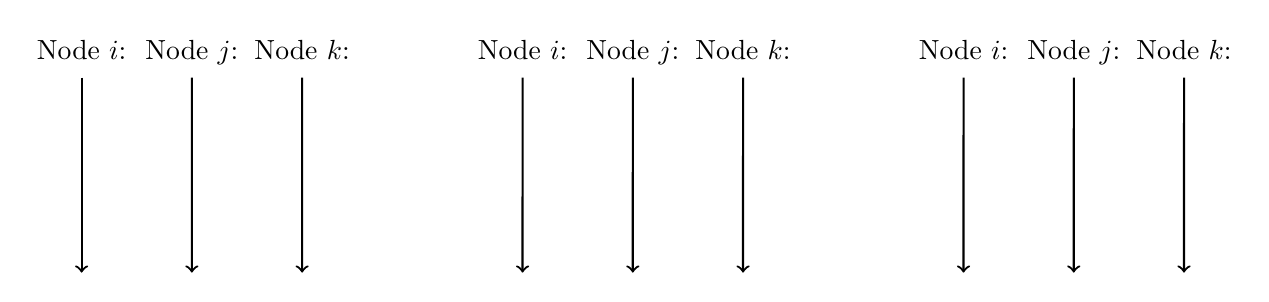
\begin{tikzpicture}[auto,scale=1.4]

\tikzstyle{every node}=[text height=8pt,text depth=3pt]
\tikzstyle{every path}=[thick,->]

\node (i1name) at (0,2) {Node $i$:};
\node (j1name) at (1,2) {Node $j$:};
\node (k1name) at (2,2) {Node $k$:};
\draw (i1name) -- (0,0);
\draw (j1name) -- (1,0);
\draw (k1name) -- (2,0);

\node (i2name) at (4,2) {Node $i$:};
\node (j2name) at (5,2) {Node $j$:};
\node (k2name) at (6,2) {Node $k$:};
\draw (i2name) -- (4,0);
\draw (j2name) -- (5,0);
\draw (k2name) -- (6,0);

\node (i3name) at (8,2) {Node $i$:};
\node (j3name) at (9,2) {Node $j$:};
\node (k3name) at (10,2) {Node $k$:};
\draw (i3name) -- (8,0);
\draw (j3name) -- (9,0);
\draw (k3name) -- (10,0);

\end{tikzpicture}

\caption{Illustrating the happens-before relation}\label{fig.happens-before}
\end{figure}

Figure~\ref{fig.happens-before} illustrates these three cases, and the formalisation of this
definition appears in Section~\ref{sect.network}.

In practice, the happens-before relationship can be captured using vector timestamps
\cite{Schwarz:1994gl,Fidge:1988tv,Raynal:1996jl}, which are used to implement protocols for causally
ordered delivery \cite{Cachin:2011wt}. As these protocols are widely known and well understood, we
leave them out of scope for this paper.


% Total order broadcast ensures that when nodes broadcast a set of messages to other nodes on the
% network, they are delivered in the same order to all recipients. By contrast, causal ordering is a
% weaker guarantee that allows greater concurrency and thus greater nondeterminism in the network.
% However, it has the advantage that it makes no assumptions about the number of nodes that are
% online.

% TODO happens-before


% There are two families of algorithms for collaborative editing: \emph{operational transformation}
% (OT)~\cite{Ellis:1989ue,Ressel:1996wx,Oster:2006tr,Sun:1998vf,Sun:1998un,Suleiman:1998eu,Nichols:1995fd}
% and \emph{conflict-free replicated datatypes}
% (CRDTs)~\cite{Shapiro:2011wy,Roh:2011dw,Preguica:2009fz,Oster:2006wj,Weiss:2010hx,Nedelec:2013ky,Kleppmann:2016ve}.
% Both allow a document to be modified concurrently on different replicas, with changes applied
% immediately to the local copy, while asynchronously propagating changes to other replicas. The
% goal of these algorithms is to ensure that for all concurrent executions, the replicas converge
% toward the same state without any edits being lost, a property known as \emph{strong eventual
% consistency}~\cite{Shapiro:2011un}.


% CRDTs are a more recent development~\cite{Shapiro:2011un}. While OT is based on transforming
% non-commutative operations so that they have the same effect when reordered, CRDTs define operations
% in a way that makes them commutative by design, making them more amenable to peer-to-peer settings
% in which each node may apply edits in a different order. CRDTs also have attractive performance
% characteristics~\cite{Mehdi:2011ke}.

% TODO Various decentralised algorithms have been proposed and all but one (Oster 2006) have
% subsequently been shown to be incorrect.

\begin{figure}
\centering
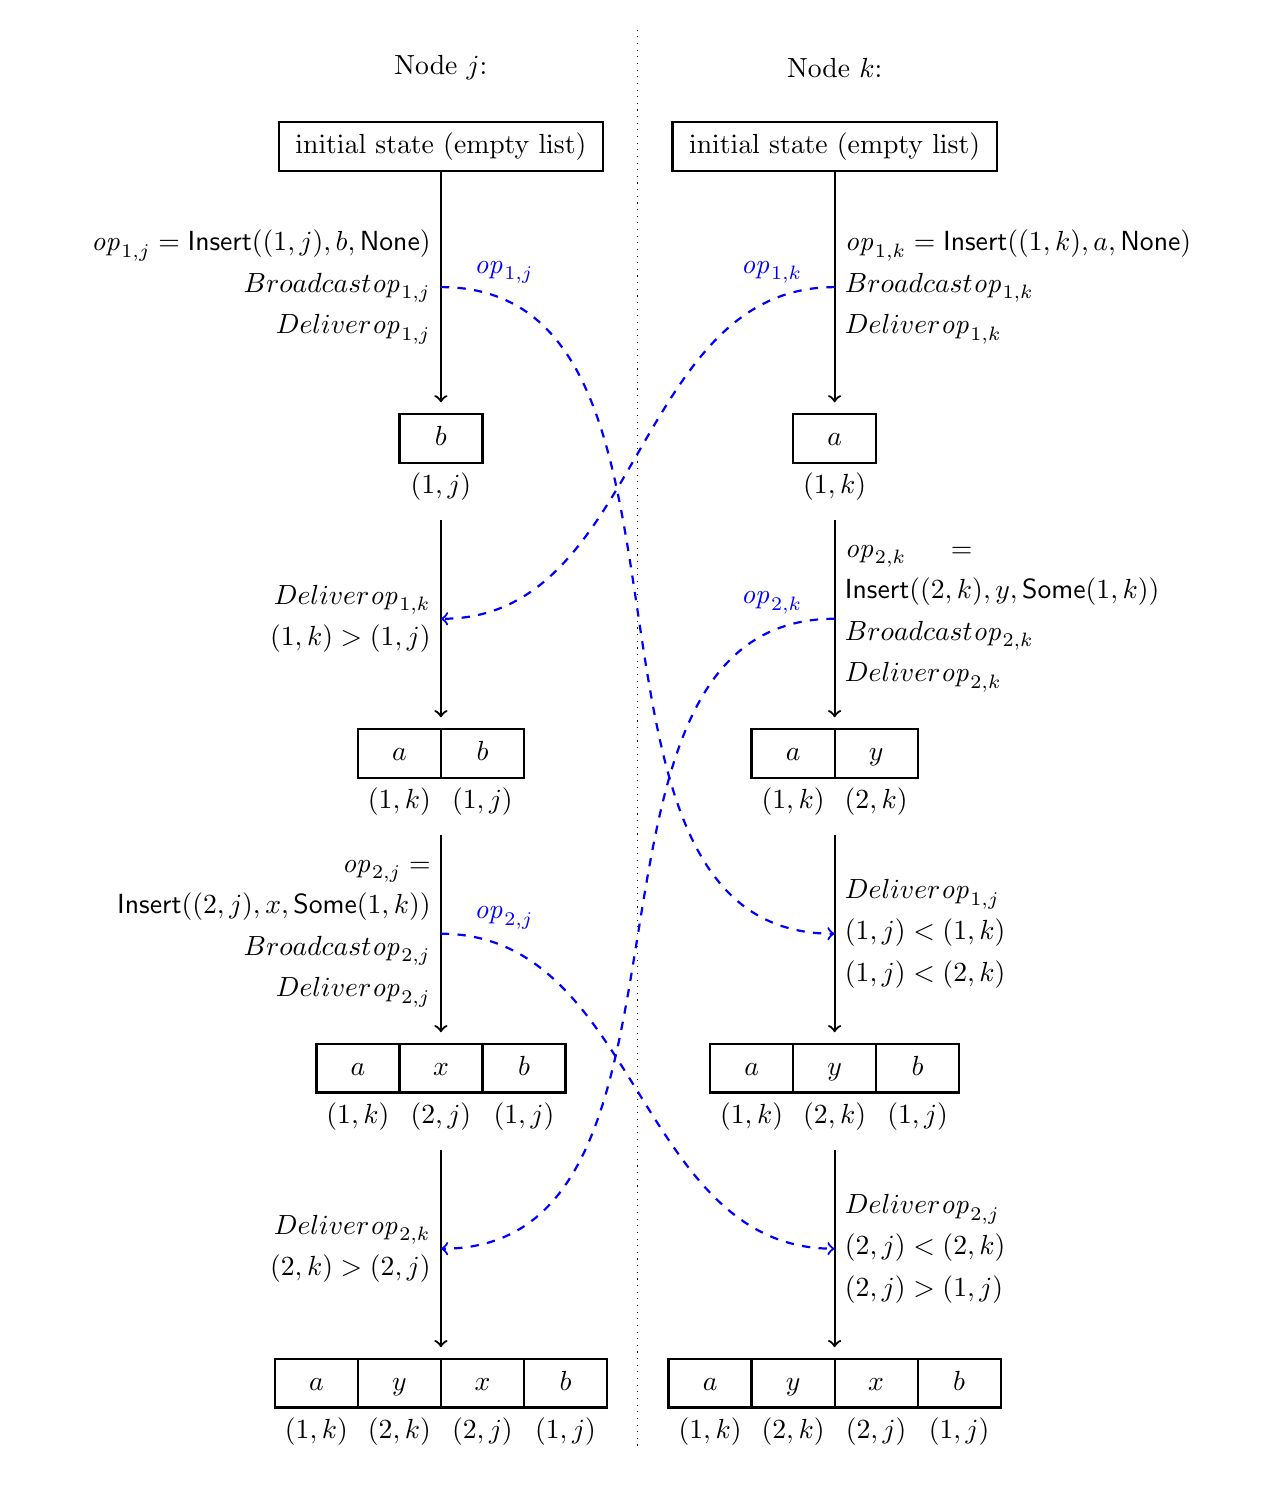
\begin{tikzpicture}[auto,scale=1.0]
\onehalfspacing
\path [draw,dotted] (2.5,-0.5) -- (2.5,17.5);

\tikzstyle{initstate}=[rectangle,draw,inner xsep=6pt,text height=8pt,text depth=3pt]
\tikzstyle{state}=[matrix,column sep={30pt,between origins}]
\tikzstyle{val}=[draw,anchor=base,minimum width=30pt,text height=8pt,text depth=3pt]
\tikzstyle{oid}=[anchor=base]
\tikzstyle{leftevent}=[left,text width=5cm,text ragged left,midway]
\tikzstyle{rightevent}=[right,text width=5cm,text ragged,midway]
\tikzstyle{every path}=[thick,->]

\node (leftR) at (0,17) {Node $j$:};
\node (left1) at (0,16) [initstate] {initial state (empty list)};
\node (left2) at (0,12) [state] {
    \node [val] {$b$};     \\
    \node [oid] {$(1,j)$}; \\
};
\node (left3) at (0,8) [state] {
    \node [val] {$a$};     & \node [val] {$b$};     \\
    \node [oid] {$(1,k)$}; & \node [oid] {$(1,j)$}; \\
};
\node (left4) at (0,4) [state] {
    \node [val] {$a$};     & \node [val] {$x$};     & \node [val] {$b$};     \\
    \node [oid] {$(1,k)$}; & \node [oid] {$(2,j)$}; & \node [oid] {$(1,j)$}; \\
};
\node (left5) at (0,0) [state] {
    \node [val] {$a$};     & \node [val] {$y$};     & \node [val] {$x$};     & \node [val] {$b$};     \\
    \node [oid] {$(1,k)$}; & \node [oid] {$(2,k)$}; & \node [oid] {$(2,j)$}; & \node [oid] {$(1,j)$}; \\
};

\draw (left1) -- (left2) node (send1j) [leftevent] {
    \hfill $\mathit{op}_{1,j} = \mathsf{Insert}((1, j), b, \mathsf{None})$ \\
    \hfill $\text{Broadcast } \mathit{op}_{1,j}$ \\
    \hfill $\text{Deliver } \mathit{op}_{1,j}$ \\
};
\draw (left2) -- (left3) node (recv1k) [leftevent] {
    \hfill $\text{Deliver } \mathit{op}_{1,k}$ \\
    \hfill $(1,k) > (1,j)$ \\
};
\draw (left3) -- (left4) node (send2j) [leftevent] {
    \hfill $\mathit{op}_{2,j} = \mathsf{Insert}((2, j), x, \mathsf{Some}(1,k))$ \\
    \hfill $\text{Broadcast } \mathit{op}_{2,j}$ \\
    \hfill $\text{Deliver } \mathit{op}_{2,j}$ \\
};
\draw (left4) -- (left5) node (recv2k) [leftevent] {
    \hfill $\text{Deliver } \mathit{op}_{2,k}$ \\
    \hfill $(2,k) > (2,j)$ \\
};

\node (rightR) at (5,17) {Node $k$:};
\node (right1) at (5,16) [initstate] {initial state (empty list)};
\node (right2) at (5,12) [state] {
    \node [val] {$a$};     \\
    \node [oid] {$(1,k)$}; \\
};
\node (right3) at (5,8) [state] {
    \node [val] {$a$};     & \node [val] {$y$};     \\
    \node [oid] {$(1,k)$}; & \node [oid] {$(2,k)$}; \\
};
\node (right4) at (5,4) [state] {
    \node [val] {$a$};     & \node [val] {$y$};     & \node [val] {$b$};     \\
    \node [oid] {$(1,k)$}; & \node [oid] {$(2,k)$}; & \node [oid] {$(1,j)$}; \\
};
\node (right5) at (5,0) [state] {
    \node [val] {$a$};     & \node [val] {$y$};     & \node [val] {$x$};     & \node [val] {$b$};     \\
    \node [oid] {$(1,k)$}; & \node [oid] {$(2,k)$}; & \node [oid] {$(2,j)$}; & \node [oid] {$(1,j)$}; \\
};

\draw (right1) -- (right2) node (send1k) [rightevent] {
    $\mathit{op}_{1,k} = \mathsf{Insert}((1, k), a, \mathsf{None})$ \\
    $\text{Broadcast } \mathit{op}_{1,k}$ \\
    $\text{Deliver } \mathit{op}_{1,k}$ \\
};
\draw (right2) -- (right3) node (send2k) [rightevent] {
    $\mathit{op}_{2,k} = \mathsf{Insert}((2, k), y, \mathsf{Some}(1, k))$ \\
    $\text{Broadcast } \mathit{op}_{2,k}$ \\
    $\text{Deliver } \mathit{op}_{2,k}$ \\
};
\draw (right3) -- (right4) node (recv1j) [rightevent] {
    $\text{Deliver } \mathit{op}_{1,j}$ \\
    $(1,j) < (1,k)$ \\
    $(1,j) < (2,k)$ \\
};
\draw (right4) -- (right5) node (recv2j) [rightevent] {
    $\text{Deliver } \mathit{op}_{2,j}$ \\
    $(2,j) < (2,k)$ \\
    $(2,j) > (1,j)$ \\
};

\begin{scope}[dashed,blue]
    \tikzstyle{every node}=[text centered]
    \draw (send1j.east) to [out=0,in=180] (recv1j.west);
    \draw (send2j.east) to [out=0,in=180] (recv2j.west);
    \draw (send1k.west) to [out=180,in=0] (recv1k.east);
    \draw (send2k.west) to [out=180,in=0] (recv2k.east);
    \node at (0.8,14.4) {$\mathit{op}_{1,j}$};
    \node at (0.8, 6.2) {$\mathit{op}_{2,j}$};
    \node at (4.2,14.4) {$\mathit{op}_{1,k}$};
    \node at (4.2,10.2) {$\mathit{op}_{2,k}$};
\end{scope}
\end{tikzpicture}

\caption{RGA example}\label{fig.two-lists}
\end{figure}


\section{Discussion}
\label{sect.discussion}

The convergence proofs for all of our CRDT implementations follow the same structure.
First we define the type of local state at each node, and the types of operations that may be invoked to modify the state.
When one node invokes an operation, it is broadcast to other nodes using our network model, implemented as a specialisation of the $\isa{network}{\isacharunderscore}\isa{with}{\isacharunderscore}(\isa{constrained}{\isacharunderscore})\isa{ops}$ locale.
An interpretation function function is called whenever a message containing an operation is delivered to a node, and it transforms that node's local state to incorporate the operation.
To demonstrate convergence, we must show that all operations commute with themselves and with each other, subject to certain assumptions.
Next, we must prove that those assumptions are always satisfied by any concurrent operations in the network.
Finally, a CRDT must demonstrate that applying an operation never fails, provided that the operation was constructed according to the definition of the algorithm.

When these proof obligations have been met, we are able to conclude that the algorithm satisfies our abstract specification $\isa{strong-eventual-consistency}$, from which we obtain convergence and progress theorems for the replicated datatype.
The abstract specification is independent of any particular network model or replication algorithm, and we assert that it constitutes a general but precise definition of strong eventual consistency.
As this recurring pattern demonstrates, we have not only isolated reusable lemmas and models of networks, but also a proof strategy that algorithm designers can use to obtain a convergence theorem for their operation-based CRDT.

By line count, over half (around 1000 lines) of our development---the network model, convergence proof, and so on---is independent from any particular CRDT and is reusable in future proofs.
In particular, we use: around 620 lines for our network model, around 380 lines for the abstract convergence proof, 775 lines for the RGA proof, around 270 lines for the ORSet proof, and around 55 lines for the Counter proof.
Additional shared code consists of around 170 lines of source.
We note here that full definitions and proofs of correctness for our three CRDT implementations are pleasingly short: all three are shown to be convergent in less than 800 lines of Isabelle source using the proof strategy described above. 

\section{Conclusion}
\label{sect.conclusion}

In this paper we adopted a ``foundational'' approach to proving the correctness of a class of SEC algorithms: Conflict-free Replicated Datatypes (CRDTs).
In our work, we made no axiomatic assumptions related to any individual algorithm; instead, we constructed a formal, realistic model of a computer network that may delay, drop, or reorder messages sent between computers---a model well known within the distributed systems community, with defensible axioms.
In addition, we isolated a formal specification of SEC, and showed that any algorithm that meets the preconditions of this specification must converge.
Our network model, the SEC specification, and a library of lemmas form a framework with which one can prove convergence for concrete CRDT implementations.

As a case study in applying our framework, we formalised three operation-based CRDTs---the Replicated Growable Array, the Observed-Remove Set, and an increment-decrement Counter.
For each algorithm we proved that its assumptions are satisfied in all possible network behaviours, and that it satisfies the preconditions of our abstract SEC specification, obtaining a guarantee that each of our three CRDT implementations converge.
Moreover, these convergence theorems were obtained using only a thin layer of CRDT-specific code, using a fixed pattern of proof in all three cases.
Since informal reasoning about convergent replication algorithms has been shown to difficult and error-prone, as exemplified by various failed proofs (Section~\ref{sect.related.verification}) and the ``a bit of a mystery'' RGA \cite{Attiya:2016kh}, we believe that their formal verification is particularly important.

Our work has been motivated by the desire to support a wider range of strong eventual consistency algorithms in distributed systems.
Operational Transformation algorithms based on the $\mathit{TP}_1$ property alone are widely used in systems such as Google Docs, but these algorithms require clients to communicate all changes via a single central server.
On the other hand, state-based CRDTs are used in systems such as Riak.
Both of these approaches are limiting.
In the case of Operational Transformation, the requirement for a central server increases the risk of faults, and prevents direct collaboration between devices via local wireless network connections.
In the case of state-based CRDTs, efficient algorithms to support complex data structures such as ordered lists are yet to be found.
Consequently, our approach provides the groundwork for a new generation of applications that use truly distributed strong eventual consistency algorithms, including robust, collaborative applications working on complex data structures in a peer-to-peer setting, something which is likely to become increasingly important in a world where mobile devices are becoming increasingly prevalent.

Although we have focussed on operation-based algorithms in this work, we speculate that our framework is also amenable to formalising Operational Transformation algorithms and state-based CRDTs.
We also speculate that our framework could be used to demonstrate the equivalence of classes of strong eventual consistency algorithms.
We leave this to future work.

%% contents of acknowledgement section are automatically suppressed when the 'anonymous' documentclass option is set
\begin{acks}
    %% Commands \grantsponsor{<sponsorID>}{<name>}{<url>} and \grantnum[<url>]{<sponsorID>}{<number>}
    %% should be used to acknowledge financial support and will be used by metadata extraction tools.
    The authors wish to acknowledge the support of the~\grantsponsor{GS501100000266}{EPSRC}{http://dx.doi.org/10.13039/501100000266} ``REMS: Rigorous Engineering for Mainstream Systems'' programme grant (\grantnum{GS501100000266}{EP/K008528}),
    the~\grantsponsor{GS501100000266}{EPSRC}{http://dx.doi.org/10.13039/501100000266} ``Interdisciplinary Centre for Finding, Understanding and Countering Crime in the Cloud'' grant (\grantnum{GS501100000266}{EP/M020320}),
    and \grantsponsor{GS100000003}{The Boeing Company}{http://dx.doi.org/10.13039/100000003}.
    We thank Peter Sewell and Alan Mycroft for constructive comments on an earlier version of this paper.
\end{acks}

\pagebreak

\bibliography{references}{}
\end{document}
